% Options for packages loaded elsewhere
\PassOptionsToPackage{unicode}{hyperref}
\PassOptionsToPackage{hyphens}{url}
%
\documentclass[
  10pt,
  onecolumn]{article}
\usepackage{amsmath,amssymb}
\usepackage{setspace}
\usepackage{iftex}
\ifPDFTeX
  \usepackage[T1]{fontenc}
  \usepackage[utf8]{inputenc}
  \usepackage{textcomp} % provide euro and other symbols
\else % if luatex or xetex
  \usepackage{unicode-math} % this also loads fontspec
  \defaultfontfeatures{Scale=MatchLowercase}
  \defaultfontfeatures[\rmfamily]{Ligatures=TeX,Scale=1}
\fi
\usepackage{lmodern}
\ifPDFTeX\else
  % xetex/luatex font selection
  \setmainfont[]{Arial}
  \setmonofont[]{Times New Roman}
\fi
% Use upquote if available, for straight quotes in verbatim environments
\IfFileExists{upquote.sty}{\usepackage{upquote}}{}
\IfFileExists{microtype.sty}{% use microtype if available
  \usepackage[]{microtype}
  \UseMicrotypeSet[protrusion]{basicmath} % disable protrusion for tt fonts
}{}
\makeatletter
\@ifundefined{KOMAClassName}{% if non-KOMA class
  \IfFileExists{parskip.sty}{%
    \usepackage{parskip}
  }{% else
    \setlength{\parindent}{0pt}
    \setlength{\parskip}{6pt plus 2pt minus 1pt}}
}{% if KOMA class
  \KOMAoptions{parskip=half}}
\makeatother
\usepackage{xcolor}
\usepackage[left=0.8in,right=0.8in,top=0.8in,bottom=0.5in]{geometry}
\usepackage{graphicx}
\makeatletter
\def\maxwidth{\ifdim\Gin@nat@width>\linewidth\linewidth\else\Gin@nat@width\fi}
\def\maxheight{\ifdim\Gin@nat@height>\textheight\textheight\else\Gin@nat@height\fi}
\makeatother
% Scale images if necessary, so that they will not overflow the page
% margins by default, and it is still possible to overwrite the defaults
% using explicit options in \includegraphics[width, height, ...]{}
\setkeys{Gin}{width=\maxwidth,height=\maxheight,keepaspectratio}
% Set default figure placement to htbp
\makeatletter
\def\fps@figure{htbp}
\makeatother
\usepackage{svg}
\setlength{\emergencystretch}{3em} % prevent overfull lines
\providecommand{\tightlist}{%
  \setlength{\itemsep}{0pt}\setlength{\parskip}{0pt}}
\setcounter{secnumdepth}{-\maxdimen} % remove section numbering
\newlength{\cslhangindent}
\setlength{\cslhangindent}{1.5em}
\newlength{\csllabelwidth}
\setlength{\csllabelwidth}{3em}
\newlength{\cslentryspacingunit} % times entry-spacing
\setlength{\cslentryspacingunit}{\parskip}
\newenvironment{CSLReferences}[2] % #1 hanging-ident, #2 entry spacing
 {% don't indent paragraphs
  \setlength{\parindent}{0pt}
  % turn on hanging indent if param 1 is 1
  \ifodd #1
  \let\oldpar\par
  \def\par{\hangindent=\cslhangindent\oldpar}
  \fi
  % set entry spacing
  \setlength{\parskip}{#2\cslentryspacingunit}
 }%
 {}
\usepackage{calc}
\newcommand{\CSLBlock}[1]{#1\hfill\break}
\newcommand{\CSLLeftMargin}[1]{\parbox[t]{\csllabelwidth}{#1}}
\newcommand{\CSLRightInline}[1]{\parbox[t]{\linewidth - \csllabelwidth}{#1}\break}
\newcommand{\CSLIndent}[1]{\hspace{\cslhangindent}#1}
\ifLuaTeX
  \usepackage{selnolig}  % disable illegal ligatures
\fi
\IfFileExists{bookmark.sty}{\usepackage{bookmark}}{\usepackage{hyperref}}
\IfFileExists{xurl.sty}{\usepackage{xurl}}{} % add URL line breaks if available
\urlstyle{same}
\hypersetup{
  pdftitle={Nitric oxide feedback to ciliary photoreceptor cells gates a UV avoidance circuit},
  hidelinks,
  pdfcreator={LaTeX via pandoc}}

\title{Nitric oxide feedback to ciliary photoreceptor cells gates a UV
avoidance circuit}
\author{true}
\date{}

\begin{document}
\maketitle

\setstretch{1.2}
\hypertarget{abstract}{%
\subsection{Abstract}\label{abstract}}

Nitric oxide (NO) produced by nitric-oxide synthase (NOS) is a key
regulator of animal physiology. Here we uncover a function for NO in the
integration of UV exposure and the gating of a UV-avoidance circuit. We
studied UV/violet avoidance mediated by brain ciliary photoreceptors
(cPRCs) in larvae of the annelid \emph{Platynereis dumerilii}. In the
larva, NOS is expressed in interneurons (INNOS) postsynaptic to cPRCs.
UV stimulation of cPRCs triggers INNOS activation and NO production. NO
signals retrogradely to cPRCs to induce their sustained post-stimulus
activation through an unconventional guanylate cyclase. This late
activation inhibits serotonergic ciliomotor neurons to induce downward
swimming. In \emph{NOS} mutants, retrograde signalling, circuit output
and UV avoidance are defective. By mathematical modelling, we
recapitulate phototransduction and circuit dynamics in wild-type and
mutant larvae. Our results reveal how NO-mediated retrograde signalling
gates a synaptic circuit and induces short-term memory of UV exposure to
orchestrate light-avoidance behaviour.

\hypertarget{introduction}{%
\subsection{Introduction}\label{introduction}}

In nervous systems, synaptic transmission and volume transmission
together shape circuit dynamics (Bargmann and Marder, 2013). While
synaptic transmission occurs at specialised contact sites, volume
transmission is characterised by the delocalised release of diverse
diffusive neuromodulators.

Nitric oxide (NO) is one such modulator with unique physical and
signalling properties. This free radical synthesized from L-arginine by
nitric oxide synthase (NOS) is short-lived and can diffuse across
biological membranes (Cudeiro and Rivadulla, 1999; Thomas, 2015).
Canonical NO signalling involves the
Ca\textsuperscript{2+}/calmodulin-dependent activation of NOS, NO
production and diffusion, and the NO-dependent activation of soluble
guanylate cyclases (sGC) leading to cGMP production (Bredt et al., 1990;
Hölscher, 1997). Given that NOS activation is Ca\textsuperscript{2+}
dependent and NOS shows neuron-type-specific expression (Aso et al.,
2019; Gibbs and Truman, 1998; Mobley et al., 2022; Wildemann and Bicker,
1999), NO action can lead to the activity-dependent modulation of neural
circuits at specific sites (Aso et al., 2019; Jacoby et al., 2018;
Vielma et al., 2014; Wang et al., 2007) .

In the vertebrate retina, NOS is expressed in amacrine, ganglion and
other cells and the actions of NO can be diverse (Cudeiro and Rivadulla,
1999; Jacoby et al., 2018; Wang et al., 2007). For example, defective NO
signalling in NOS knockout mice leads to a decreased sensitivity of
retinal ganglion cells to light stimulation (Wang et al., 2007). In the
retina, NO signalling can also involve pathways other than canonical sGC
signalling (Jacoby et al., 2018; Tooker et al., 2013; Wei et al., 2012).
Due to the complex expression of NOS in vertebrates and the diversity of
its functions, it has been challenging to link the neurophysiological
effects of NO to signalling mechanisms and behaviour change.

In the \emph{Drosophila} brain, NO signalling is also involved in tuning
circuit activity at diverse and specific sites. In the ellipsoid body of
the central complex, NO is involved in visual working memory (Kuntz et
al., 2017). NO signalling also tunes the dynamics of associative
memories in mushroom body circuits. NOS is expressed in PPL1-γ1pedc
mushroom-body neurons where it is involved in shortening memory
retention while promoting fast memory updating in response to new
experiences (Aso et al., 2019).

In the whole organism context, NO signalling has often been studied in
diverse marine invertebrates, where NO can regulate larval settlement
and metamorphosis (Leise et al., 2001; Locascio et al., 2022; Song et
al., 2021; Ueda et al., 2016; Zhang et al., 2012). While NOS-expressing
neurons potentially responsible for these effects have been reported
(Bishop and Brandhorst, 2007; Locascio et al., 2022), it has not been
possible to link these NO-dependent effects on behaviour or life-cycle
transitions to neuronal activity and function.

Overall, we still know little about how NO production relates to
stimulus conditions, how it shapes circuit activity at specific neuron
types, and how NO-dependent modulation relates to behaviour.

To investigate NO function in neural circuit dynamics and behaviour,
here we study larvae of the marine annelid model \emph{Platynereis
dumerilii} (Ozpolat et al., 2021). \emph{Platynereis} has emerged as a
model for systems neuroscience with a toolkit that enables the
combination of behavioural analysis and neuronal activity imaging with
genetic manipulations. A whole-body synaptic connectome and gene
expression atlases are also available and can be integrated with
functional approaches in live animals thanks to the cellular-level
stereotypy of larvae of the same developmental stage (Ozpolat et al.,
2021; Verasztó et al., 2020; Verasztó et al., 2017; Vergara et al.,
2021).

We uncovered an essential function for NO signalling in larval
UV/violet-light avoidance behaviour. In \emph{Platynereis} larvae,
UV/violet avoidance is mediated by brain ciliary photoreceptor cells
(cPRCs) and is characterised by downward swimming (Verasztó et al.,
2018). The cPRCs express a ciliary-type opsin, c-opsin1 (Arendt et al.,
2004) that forms a UV-absorbing bistable photopigment with an absorption
maximum around 384 nm (Tsukamoto et al., 2017; Veedin Rajan et al.,
2021; Verasztó et al., 2018). Upon UV/violet exposure, the cPRCs show a
characteristic biphasic Ca\textsuperscript{2+} response that is c-opsin1
dependent. UV/violet avoidance is also c-opsin1 dependent and is
defective in \emph{c-opsin1} mutants (Verasztó et al., 2018). Here we
show that \emph{Platynereis} NOS is expressed in interneurons of the
cPRC circuit and is required for UV/violet-avoidance. By combining
Ca\textsuperscript{2+} imaging across the fully-mapped cPRC circuit
(Verasztó et al., 2018) with genetic perturbations and mathematical
modelling, we describe how NO tunes circuit dynamics through
non-synaptic retrograde signalling to cPRCs. This delayed neuroendocrine
feedback integrates UV/violet exposure to induce a short-term memory
manifested in altered circuit activity and an aversive behavioural
response.

\hypertarget{results}{%
\subsection{Results}\label{results}}

\textbf{Nitric oxide synthase is expressed in interneurons of the
UV-avoidance circuit}

We identified a single \emph{nitric oxide synthase} (\emph{NOS}) gene in
the \emph{Platynereis dumerilii} genome and transcriptome data.
Phylogenetic analysis of NOS proteins indicate that \emph{Platynereis}
NOS belongs to an orthology group of bilaterian NOS sequences (Figure
1---figure supplement 1). To characterise the expression pattern of
\emph{NOS}, we used in situ hybridization chain reaction (HCR) and
transient transgenesis. In two- and three-day-old larvae, we detected
\emph{NOS} expression in four cells (two of them weakly expressing) in
the apical organ region (Figure 1D and Figure 1---figure supplement 2).
\emph{NOS} was also expressed in the region of the visual eyes (adult
eyes) and the pigmented eyespots (Figure 1---figure supplement 2). The
four apical organ cells, but not the eyes, were also labelled with a
\emph{NOS} reporter construct driving palmitoylated tdTomato (Figure
1E). This reporter also revealed the axonal projections of these central
NOS-expressing neurons. The position and morphology of the four
\emph{NOS+} cells allowed us to identify the same four cells as four
interneurons (INNOS) in our three-day-old whole-body \emph{Platynereis}
volume EM data (Verasztó et al., 2020; Williams et al., 2017) (Figure
1B,C). In the synaptic connectome, the INNOS cells are postsynaptic to
the UV-sensory cPRCs and presynaptic to the INRGWa interneurons, which
are also cPRC targets (Figure 1C, F). The projections of INNOS cells are
segregated into input (dendritic) and output (axonal) compartments, with
cPRC inputs occurring on the dendritic part in the dense neurosecretory
plexus. INNOS output-synapses form in the more ventral projection region
(Figure 1---figure supplement 3). INRGWa neurons synapse on the head
serotonergic ciliomotor neurons (Ser-h1), which synapse on the
cholinergic MC ciliomotor neuron and cells of the prototroch ciliary
band (Figure 1C, F) (Verasztó et al., 2017).

\begin{figure}
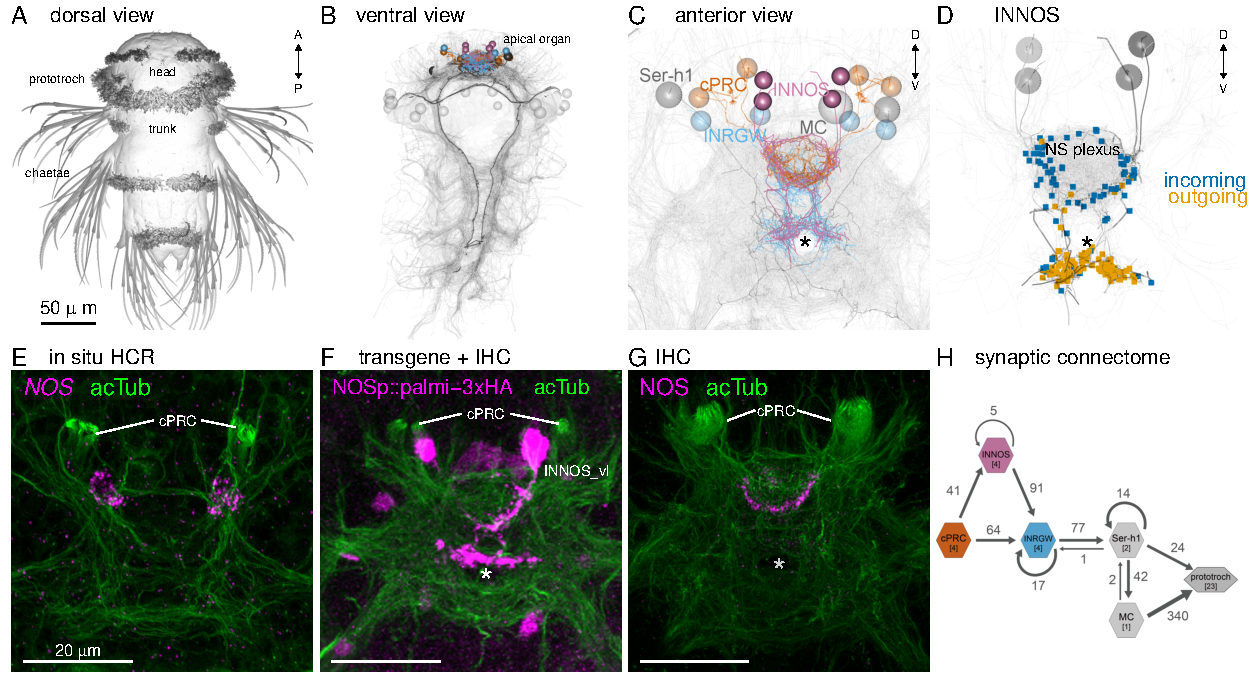
\includegraphics[width=25in]{figures/Fig1} \caption{**Figure 1. Identification of *NOS*-expressing interneurons (INNOS) within the cPRC circuit.** **(A)** Scanning electron microscopy image of a three-day-old *Platynereis* larva. **(B, C)** Volume rendering of the neuron types (cPRC, INNOS, INRGWa, Ser-h1 and MC) in the cPRC circuit reconstructed from a whole-body transmission electron microscopy volume of a three-day-old larva. Neurite skeletons are shown with cell-body positions represented by spheres. Projections of all neurons in the body are shown in grey to highlight the neuropils. The outline of the yolk is also indicated in grey. In B, nuclei positions of the prototroch head ciliary band are shown as grey spheres. **(D)** Expression of the *NOS* gene detected by in situ HCR (magenta) in a two-day-old larva (anterior view). Antibody staining for acetylated α-tubulin (acTub: green) highlights cPRC cilia and the neuropil. **(E)** Expression of a *NOS* reporter (NOSp::palmi-3xHA; magenta) labelled with an anti-HA antibody in a two-day-old larva (anterior view). Antibody staining for acetylated α-tubulin (acTub; green) highlights cPRC cilia and the neuropil. **(F)** Synaptic wiring diagram of the cPRC circuit. Hexagons represent cell groups, with the number of cells per group shown in square brackets. Arrows represent the summed number of synaptic contacts between cell groups. Arrow thickness is proportional to the number of synapses.}\label{fig:unnamed-chunk-1}
\end{figure}

\textbf{Nitric oxide is produced during UV/violet stimulation of the
cPRCs}

The expression of \emph{NOS} in the INNOS interneurons in the cPRC
circuit suggests that NO signalling may be involved in
UV/violet-avoidance. To test this, first we asked whether NO is produced
during UV/violet stimulation of the larvae. We injected the fluorescent
NO-reporter DAF-FM into zygotes and imaged two-day-old larvae while
exposing the region of cPRC cilia to 405 nm violet light. To mark cell
outlines, we coinjected mRNA encoding a red-fluorescent reporter
(RGECO), allowing the identification of the cPRCs. Following light
stimulation in the region of the ramified cilia of the cPRCs, we
detected an increase in DAF-FM fluorescence in the anterior
neurosecretory neuropil, the region of INNOS projections. This increase
did not occur in larvae in which we illuminated a control area (Figure
2).

\begin{figure}
\includegraphics[width=29.17in]{figures/Fig2} \caption{**Figure 2. NO produced by UV/violet stimulation to cPRCs.** (**A**) DAF-FM fluorescence in the region of the neurosecretory neuropil. The white line indicates the outline of the larva. The dashed line corresponds to the area where fluorescence was quantified. The circles indicate the location of cPRC and control stimulation. The cPRCs are marked by thin lines. (**B**) DAF-FM fluorescence before and during 405 nm light stimulation. (**C**) Changes in DAF-FM fluorescence over time during 405 nm stimulation of the cPRCs or a control area (ctr stim.). The purple box indicates the duration of 405 nm stimulation. Individual normalized traces (ΔF/F0) are shown as thin lines. Thick lines show the mean value with 0.95 confidence intervals. N = 9 larvae for control and 11 for cPRC stimulation. <br> Figure 2 -- source data 1. DAF-FM fluorescence reads.}\label{fig:unnamed-chunk-2}
\end{figure}

\textbf{Nitric oxide signalling mediates UV-avoidance behaviour}

We next tested whether NO signalling regulates UV/violet avoidance. To
achieve this, we generated two \emph{Platynereis} \emph{NOS} knockout
lines using the CRISPR/Cas9 method. We recovered two deletions
(NOSΔ11/Δ11 and Δ23/Δ23), both frame-shift mutations leading to an early
stop codon and thus likely representing null alleles (Figure 3---figure
supplement 1A). We could establish a homozygous line for both mutations
indicating that NOS is not an essential gene in \emph{Platynereis}. To
quantify UV avoidance, we recorded the trajectories of freely swimming
wild type and mutant larvae in vertical columns, illuminated laterally
from two opposite sides with 395 nm UV light (Figure 3A and Figure
3---figure supplement 1B). As previously shown, wild-type larvae swim
downward following non-directional UV/violet light stimulation (Verasztó
et al., 2018). In contrast, both two- and three-day-old homozygous
\emph{NOS}-mutant larvae showed a strongly diminished UV-avoidance
response (Figure 3A, B and Figure 3---figure supplement 1B, C). This
phenotype is similar to the defective UV-avoidance of \emph{c-opsin1}
mutant larvae (Verasztó et al., 2018) and reveals a requirement for NOS
in UV-avoidance behaviour. Wild type but not mutant larvae also showed
an increase in swimming speed under UV light that may be due to downward
swimming trajectories (swimming in the direction of gravity) (Figure 3B
and Figure 3---figure supplement 1C). We also tested directional
phototaxis, by exposing larvae to 480 nm directional collimated light
from the top of the column. Three-day-old but not two-day-old
\emph{NOS}-mutant larvae also showed reduced phototactic behaviour,
suggesting a function for \emph{NOS} in the visual eyes that mediate
three-day-old phototaxis (Randel et al., 2014) (Figure 3D and Figure
3---figure supplement 1G).

To distinguish between an acute and developmental function of NOS in
light responses, we also tested larvae exposed to the NOS inhibitor
L-NAME. Larvae incubated for 5 min in 0.1 mM or 1 mM L-NAME showed a
dose-dependent inhibition of UV avoidance. In contrast, phototaxis was
not affected (Figure 3C, E). Overall, our results indicate an acute
requirement for NOS signalling in UV-avoidance and a possible indirect,
developmental role in the visual system, reminiscent of the function of
NO signalling in \emph{Drosophila} eye development (Gibbs and Truman,
1998).

\begin{figure}
\includegraphics[width=33.33in]{figures/Fig3} \caption{**Figure 3. NOS is required for UV avoidance in *Platynereis* larvae.**  (**A**) Swimming trajectories of wild type (WT, n=32) and *NOS* mutant (*NOSΔ11/Δ11*, n=26 and *NOSΔ23/Δ23*, n=47) three-day-old larvae. All trajectories start at 0 x and y position and time 0 corresponding to 10 sec after the onset of 395 nm stimulation from the side. (**B**) Vertical position of batches of wild type and mutant three-day-old larvae over time under 395 nm UV stimulation. The starting position of each larval trajectory was set to 0. (**C**) Vertical position of batches of control and L-NAME-treated (0.1 and 1 mM) three-day-old larvae over time under 395 nm UV stimulation. The starting position of each larval trajectory was set to 0. (**D**) Vertical displacement in 30 sec bins of wild type and mutant (*NOSΔ11/Δ11* and *NOSΔ23/Δ23*) three-day-old larvae stimulated with 395 nm light from the side, 488 nm light from the top and 395 nm light from the top. (**E**) Vertical displacement in 30 sec bins of control and L-NAME-treated (0.1 and 1 mM) three-day-old larvae stimulated with 395 nm light from the side, 488 nm light from the top and 395 nm light from the top. <br> Figure 3 -- source data 1-5. Source data for panels A-E.}\label{fig:unnamed-chunk-3}
\end{figure}

\textbf{NO retrograde signalling tunes cPRC responses to UV/violet
stimulation}

To investigate how NO signalling alters the dynamics of the cPRC
circuit, we carried out Ca\textsuperscript{2+} imaging experiments. We
ubiquitously expressed the Ca\textsuperscript{2+} sensor GCaMP6s in
larvae and imaged Ca\textsuperscript{2+} signals during 405 nm
stimulation of the cPRCs. As we have shown previously, a 20 sec local
stimulation of cPRC cilia led to a transient increase in cPRC
Ca\textsuperscript{2+} levels, followed by a transient decrease
(Verasztó et al., 2018). After \textasciitilde20-sec,
Ca\textsuperscript{2+} levels in cPRCs were raising again, reaching
higher levels than at the start of the stimulus -- a response that may
involve cPRC depolarisation (Figure 4A, B). This activation phase occurs
after the 20 sec stimulation period and is likely due to a delayed
neuroendocrine feedback (Verasztó et al., 2018). To determine whether NO
mediates such a feedback, we repeated the experiment in
\emph{NOS}-mutant larvae. While we detected the initial activation phase
followed by inhibition, in homozygous \emph{NOS}-mutants for both CRISPR
alleles this was not followed by delayed activation. Instead,
Ca\textsuperscript{2+} levels dropped to a low steady-state level
(Figure 4A, B). We thus identified a requirement for NO signalling in
the late-phase activation of cPRCs.

\textbf{Two unconventional guanylate cyclases are expressed in the
cPRCs}

Next we aimed to identify the NO receptor in the cPRCs. NO generally
acts via soluble guanylate cyclases (sGC), belonging to the guanylate
cyclase family with a CYC domain (PFAM domain: PF00211). NO binding to
the heme group of sGC leads to increased cyclic guanosine monophosphate
(cGMP) production. Analysis of sGCs in \emph{Platynereis} indicated that
these genes are not expressed in any of the cells of the cPRC circuit
(not shown and (Verasztó et al., 2017)). Recently, Moroz and coworkers
reported an atypical but widely conserved family of guanylate cyclases
with a NIT (nitrite/nitrate sensing) domain (PF08376) (NIT-GC) as
potential mediators of NO signalling (Moroz et al., 2020). To identify
NIT-GCs in \emph{Platynereis}, we searched transcriptome resources and
retrieved 15 potential NIT-GC homologs (Figure 4---figure supplement 1
and 2). To analyse the relationship of these sequences to metazoan
NIT-GCs, we retrieved protein sequences with a CYC domain from the
transcriptome and genome databases of 45 metazoan and 2 choanoflagellate
species. We carried out cluster analysis and phylogenetic reconstruction
on a group of membrane-bound guanylate cyclases with sGCs as an
outgroup. In agreement with Moroz et al. (Moroz et al., 2020), we found
a group of GCs with NIT domains with representatives in placozoans,
cnidarians, some ecdysozoans, echinoderms, and lophotrochozoans. The 15
\emph{Platynereis} sequences belonged to several deeply diverged clades
in the phylogenetic tree (Figure 4---figure supplement 1 and 2).

To characterise the expression of NIT-GCs, we used previously published
spatially-mapped single-cell transcriptome data (Achim et al., 2015;
Williams et al., 2017). Among the 15 NIT-GCs, two showed high and
specific expression in the cPRCs and one was expressed in the INNOS
cells (Figure 4---figure supplement 2). In the single-cell data, we
could identify the cPRCs by the specific expression of the markers
\emph{c-opsin1} and the \emph{pedal-peptide2 neuropeptide precursor}
(\emph{MLD proneuropeptide}) (Arendt et al., 2004; Williams et al.,
2017) (Figure 4---figure supplement 3A). The INNOS cells were identified
by NOS expression and spatial mapping in the brain (Achim et al., 2015).
We decided to focus on two NIT-GCs expressed in the cPRCs and with a
full-length sequence, \emph{NIT-GC1} and \emph{NIT-GC2}. To confirm the
single-cell data, we first carried out in situ hybridisation chain
reaction (HCR) with probes for \emph{NIT-GC1} and \emph{NIT-GC2} mRNA.
Both genes were specifically expressed in the four cPRCs, as confirmed
by co-labeling with an acetylated α-tubulin antibody and with an HCR
probe against \emph{pedal peptide 2/MLD proneuropeptide} (Figure 4C, D
and Figure 4---figure supplement 3A-C). To analyse the subcellular
localisation of NIT-GC1 and NIT-GC2 at the protein level, we raised and
affinity-purified polyclonal antibodies against a specific peptide
sequence from both proteins. In immunostainings, we found that NIT-GC1
was localise to the region corresponding to the axonal projections of
the cPRCs in the anterior neurosecretory plexus (Figure 4E).
Co-immunostaining with the rabbit NIT-GC1 antibody and a custom rat
antibody raised against \emph{Platynereis} NOS revealed the localisation
of both proteins in dots in the neurosecretory neuropil (Figure
4---figure supplement 3D). In contrast, NIT-GC2 specifically labelled
the ramified sensory cilia of the cPRCs (Figure 4F). These different
subcellular localisations suggest that the two NIT-GCs are involved in
different intracellular signalling processes in the ciliary and axonal
regions of the cPRCs.

\textbf{NIT-GC1 produces cGMP in an NO-dependent manner}

To further characterise these atypical guanylate cyclases, we focused on
NIT-GC1 and carried out in vitro experiments. In bacteria, NIT domains
are thought to regulate cellular functions in response to intra- or
extracellular nitrate and nitrite. NIT-GC1 has a NIT domain and a highly
conserved cyclase domain that is expected to catalyse cGMP synthesis
(Figure 4G). The NIT domain may render NIT-GC1 dependent on NO signals.
To test this, we co-expressed the cGMP indicator Green cGull (Matsuda et
al., 2016) and NIT-GC1 in cultured COS-7 (monkey kidney) cells, a cell
line with minimal endogenous sGC activity (Matsuda et al., 2016). For
balanced expression, we used a single plasmid with the two open-reading
frames separated by the 2A self-cleaving peptide (Figure 4H).
Application of the NO donor SNAP lead to increased Green cGull
fluorescence, an effect we did not observe when cells were exposed to
DMSO or when Green cGull was expressed alone (Figure 4I-K). To test
whether this effect is dependent on the NIT domain, we also tested a
deletion construct of NIT-GC1 lacking the NIT domain (Figure 4G). Cells
expressing this construct and Green cGull did not show an increased
fluorescence of the cGMP reporter when exposed to SNAP (Figure 4L).
These results indicate that NIT-GC1 is able to catalyse cGMP production
in an NO-dependent manner and this function requires the NIT domain.
These results establish NIT-GC1 as a biochemical sensor of NO or its
derivatives.

\textbf{NIT-GC1 is required for NO-mediated retrograde signalling to
cPRCs during the UV response}

To test the in vivo function of NIT-GC1 and NIT-GC2 in cPRC responses,
we combined Ca\textsuperscript{2+} imaging with morpholino-mediated
knockdowns. We used two translation-blocking morpholinos for each
\emph{NIT-GC} gene and tested knockdown efficiency by immunostaining
injected animals with the NIT-GC1 and NIT-GC2 antibodies (Figure
4---figure supplement 3E,F). For both genes, the morpholinos led to a
strong reduction in the respective antibody signal, confirming efficient
knockdown and antibody specificity.

In NIT-GC1 morphant larvae, the delayed activation of cPRCs following
405 nm stimulation did not occur (Figure 4M). This phenotype is similar
to the phenotype of \emph{NOS} mutants suggesting that NIT-GC1 acts as
the NO sensor in cPRCs to drive their delayed activation. This could
occur via increased cGMP production and the opening of a
cyclic-nucleotide-gated ion channel (CNG) specific to cPRCs (Tosches et
al., 2014). NIT-GC2 morphant larvae, in contrast, showed a step-up
increase in Ca\textsuperscript{2+} following light stimulation (Figure
4N). The Ca\textsuperscript{2+} signal decayed during stimulation and
was off after light off. These data support an essential role for
ciliary-localised NIT-GC2 in suppressing cPRC Ca\textsuperscript{2+}
following its transient rise at stimulus onset. Overall, these knockdown
experiments revealed different signalling mechanisms for the two NIT-GCs
that may be due to their different subcellular localisations.

\begin{figure}
\includegraphics[width=38.89in]{figures/Fig4} \caption{**Figure 4. NOS and two NIT-GCs shape Ca^2+^ signals during cPRC UV/violet response.** (**A**, **B**) GCaMP6s signals in cPRCs in wild type and *NOS* mutant (A, *NOSΔ11/Δ11*, B, *NOSΔ23/Δ23*) larvae during 405 nm light stimulation. (**C**, **D**) In situ HCR for (C) *NIT-GC1* and (D) *NIT-GC2* (magenta) in three-day-old *Platynereis* larvae. Larvae were co-stained with an antibody against acetylated α-tubulin to label cPRC cilia and the neuropil (green). (**E**, **F**) Immunostaining for (E) NIT-GC1 and (F) NIT-GC2 (magenta), co-stained for acetylated α-tubulin (green). (**G**) The domain structure of *Platynereis* NIT-GC1 and the truncated NIT-GC1ΔNIT protein lacking the NIT domain. A predicted transmembrane region (TM) is shown in grey. (**H**) Schematic of the cell-based assay to detect cGMP production following the addition of an NO donor SNAP or DMSO as control. (**I**-**L**) Green cGull fluorescence over time for the four conditions tested. Individual responses and their mean with 0.95 confidence interval are shown (n > 6 cells). Intensities are normalized (ΔF/F0). The indicated chemicals were added at 2 min after the start of imaging (grey bars). (**M**, **N**) GCaMP6s signals in cPRCs in (M) NIT-GC1 and (N) NIT-GC2 morphant larvae during 405 nm light stimulation. Individual responses and their mean with 0.95 confidence interval are shown. <br> Figure 4 -- source data 1-8. Source data for panels A, B and I-N.}\label{fig:unnamed-chunk-4}
\end{figure}

\textbf{NO signalling shapes the dynamics of the cPRC circuit}

To investigate how NO and NIT-GC signalling influence the dynamics of
the cPRC circuit, we imaged Ca\textsuperscript{2+} signals from
postsynaptic neurons in wild type, mutant and morphant larvae. We were
able to image the activity of all neurons in the cPRC circuit (INNOS,
INRGWa, Ser-h1 and MC). The MC cell was identified based on its position
and intrinsic activity (Verasztó et al., 2017). To unambiguously
identify all other cells from which we recorded Ca\textsuperscript{2+}
signals, we developed an on-slide immunostaining method (Figure
5---figure supplement 1A). We used the cell-specific antibody markers
against RYamide (INNOS) (Figure 5---figure supplement 1B-D), RGWamide
(INRGWa) and serotonin (Ser-h1) (Conzelmann et al., 2011) to immunostain
agar-embedded larvae following Ca\textsuperscript{2+} imaging. Based on
the position of the nuclei, we could correlate live and fixed samples at
a single-cell precision (Figure 5A, B). Due to the stereotypy of the
larvae, we could also identify neurons based on their position and
Ca\textsuperscript{2+} activity in activity-correlation maps (Figure
5C).

We first quantified the responses of the INNOS and INRGWa interneurons
during 405 nm stimulation of the cPRCs. In both wild type and
\emph{NOS}-mutant larvae, INNOS cells showed an increase in
Ca\textsuperscript{2+} during stimulation (Figure 5D). In contrast, the
INNOS response was flat or slightly negative in NIT-GC2 morphant larvae
(Figure 5E) revealing an essential role for NIT-GC2-mediated cPRC
suppression in INNOS activation. The INRGWa cells were initially
inhibited during cPRC stimulation, followed by a delayed activation
paralleling the second activation phase of the cPRCs. This late INRGWa
response was lacking in \emph{NOS}-mutants (Figure 5F). In NIT-GC2
morphants, INRGWa cells showed a transient increase in
Ca\textsuperscript{2+} that decayed after light off and a delayed
activation was not present (Figure 5G).

Next, we imaged Ca\textsuperscript{2+} signals from Ser-h1 and MC
neurons in wild type and \emph{NOS} mutant larvae. Ser-h1 cells showed
an activation profile that correlated with cPRC activity, including a
reduction in Ca\textsuperscript{2+} during stimulation followed by a
rebound, a response that was defective in \emph{NOS} mutants (Figure
5I). The MC cell showed sustained activation, including a late-phase
that was lacking in \emph{NOS} mutants (Figure 5I). These data suggest
that during 405 nm stimulation the Ser-h1 cells are inhibited and the MC
cell is activated, and this regulation is NO-dependent. This pattern is
expected to inhibit ciliary activity in the prototroch but not in the
other ciliary bands (with no Ser-h1 or MC synapses), triggering
NO-dependent downward swimming.

\begin{figure}
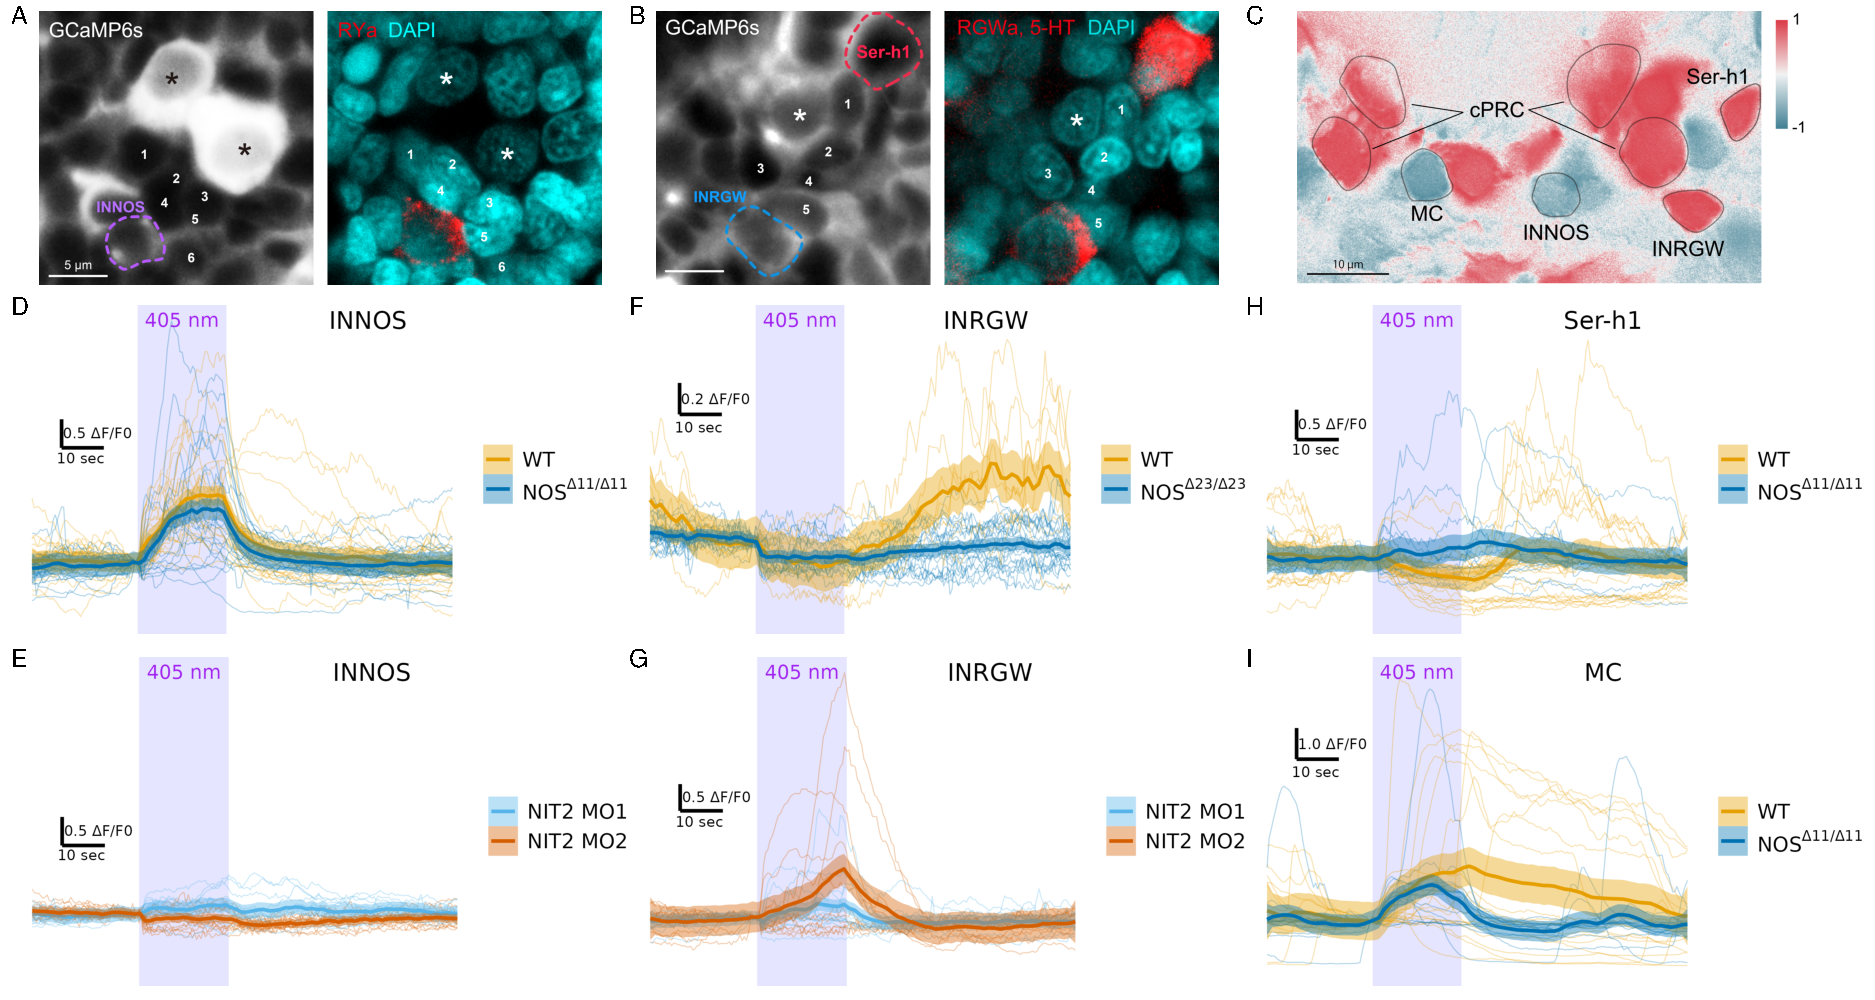
\includegraphics[width=52.08in]{figures/Fig5} \caption{**Figure 5. NOS- and NIT-GC2-dependent dynamics of the cPRC circuit.** (**A, B**) GCaMP6s imaging from cPRCs and INNOS cells (left panels) followed by on-slide immunostaining for (A) RYamide to label INNOS and (B) RGWamide+serotonin to label INRGWa and Ser-h1 (red). Nuclei are stained with DAPI (cyan). Asterisks indicate cPRC nuclei. Numbers mark the same cells in the GCaMP and immunostaining images matched by position. (**C**) Correlation map of neuronal activity of the cPRCs, INNOS, INRGWa, Ser-h1 and MC neurons. (**D**) GCaMP6s fluorescence in INNOS cells in wild type (WT) and *NOSΔ11/Δ11* mutant larvae during 405 nm stimulation of the cPRC cilia. (**E**) GCaMP6s fluorescence in INNOS cells in NIT-GC2 morphant larvae during 405 nm stimulation. (**F**) GCaMP6s fluorescence in INRGWa cells in wild type and *NOSΔ23/Δ23* mutant larvae during 405 nm stimulation. (**G**) GCaMP6s fluorescence in INRGWa cells in NIT-GC2 morphant larvae during 405 nm stimulation. (**H, I**) GCaMP6s fluorescence in (H) Ser-h1 cells and (I) the MC cell in wild type and *NOSΔ11/Δ11* mutant larvae during 405 nm stimulation. <br> Figure 5 -- source data 1-6. Source data for panels D-I.}\label{fig:unnamed-chunk-5}
\end{figure}

\textbf{Mathematical modelling of cPRC-circuit dynamics}

To further analyse the dynamics of responses to UV light and formally
describe cPRC phototransduction, synaptic connections and NO retrograde
signalling, we developed a mixed cellular-circuit-level mathematical
model. We used our Ca\textsuperscript{2+} imagining data of cPRC, INNOS
and INRGWa cells collected in wild type, \emph{NOS} knockout and
\emph{NIT-GC2} morphant larvae to formulate assumptions that are the
basis of the proposed model.

We modeled a direct c-opsin1-dependent response to UV leading to the
initial rise in Ca\textsuperscript{2+} levels. The mechanism of this
signal is not known but may include Gα and Gβ signalling, CNGAα channel
activation or other pathways. We further assumed that in cPRC cells,
Ca\textsuperscript{2+} levels increase with cGMP. We modeled a decrease
in cGMP and Ca\textsuperscript{2+} levels due to a NIT-GC2-dependent
pathway (Figure 6A). The effect of NO in cPRC cells is captured by
another term that describes a NIT-GC1 and NO-dependent increase in cGMP.
Based on the synaptic connectome, we infered a feedforward coupling
between cPRC cells and INNOS and INRGWa cells. The proposed synaptic
coupling is UV-dependent, decays linearly and is suppressed in NIT-GC2
morphants (Figure 6A).

In the INNOS cells, we assumed that excitatory synaptic input from cPRC
(or rebound from tonic inhibition) leads to a rise in
Ca\textsuperscript{2+} leading to NO production via NOS. This input is
NIT-GC2-dependent. In the INRGWa cells, we modeled a decrease in
Ca\textsuperscript{2+} based on an inhibitory UV-dependent synaptic
signal from the cPRCs. We further assumed the existence of direct
excitatory coupling between cPRC Ca\textsuperscript{2+} levels and
INRGWa Ca\textsuperscript{2+} to account for the late effects of cPRC on
INRGWa (Figure 6A). The UV-dependent and
Ca\textsuperscript{2+}-dependent signals may be mediated by different
transmitters released by cPRCs during distinct phases of their
activation cycle. In addition, we assumed a direct inhibitory coupling
between INNOS Ca\textsuperscript{2+} and INRGWa Ca\textsuperscript{2+}.
Finally, in all variables, we assumed a linear decay and constant
production to set a steady state (Figure 6A). Since the aim of the model
is to capture the normalised fluorescence data, the model is
nondimensionalised. UV stimulation is modelled as a square pulse. To
find model parameters producing an output fitting the experimental data
we employed a global optimisation method known as a genetic algorithm
(GA).

Through this optimisation procedure, we found parameters that gave a fit
to our experimental data under all conditions (Figure 6B; Figure
6--figure supplement 1-5). We could fit to mean Ca\textsuperscript{2+}
profiles but also individual Ca\textsuperscript{2+} transients. Our
model only includes a minimal set of parameters and assumptions of
interactions that are required to describe the dynamics of cPRC, INNOS
and INRGWa in wild type and loss-of-function conditions (Figure 6A, B).
The model highlights that cPRC phototransduction employs distinct
pathways that operate on different time scales and differentially
influence cPRC Ca\textsuperscript{2+} levels. The coupling between cPRCs
and interneurons also requires different signalling mechanisms, either
through distinct neurotransmitters or receptors expressed in the
different cells.

To identify possible molecular pathways, we analysed single-cell
transcriptome data for cPRC, INNOS and INRGWa identified by spatial
mapping (Achim et al., 2015) and unique marker genes (Williams et al.,
2017). In cPRCs, we found transporters and synthetic enzymes indicating
cholinergic, glutaminergic, glycinergic, GABAergic and adrenergic
neurotransmission (Figure 6C). For each neurotransmitter, we also found
receptor-encoding genes expressed in INNOS and INRGWa (Figure 6C). The
two types of interneurons often expressed different subunits or types of
these receptors, indicating differential signalling (Figure 6C).

Based on these data, our experimental results and the mathematical
model, we assembled a minimal phototransduction and circuit diagram. The
components for which experimental data are available are shown in bold.
Other potential molecular players are also indicated (Figure 6D).

\begin{figure}
\includegraphics[width=25in]{figures/Fig6} \caption{**Figure 6. Mathematical modelling and signalling mechanisms of the cPRC circuit.** (**A**) Diagram of the mathematical model with the componenets, interactions, parameters and equations used to model Ca^2+^ dynamics. (**B**) Average Ca^2+^ traces (upper) and traces from model simulations (lower) fitted to the data. (**C**) Dot plot of genes (columns) expressed in three types of cells (rows) in the cPRC circuit using single cell RNA-Seq. The size of the dots is expressed in proportion to the percentage of cells expressing that gene relative to all cells. The colours represent the normal logarithm of the number of transcripts in the cells expressing the gene. (**D**) Schematic diagram of the signalling pathway of the cPRC circuit, focusing on the NO feedback. <br> Figure 6 -- source data 1. TPM values for each gene and the percentage of expressed genes.}\label{fig:unnamed-chunk-6}
\end{figure}

To generate new insights from the model, we asked how the duration and
intensity of UV stimulation influences signalling output, measured as
the magnitude (quantified as area under peak, AUP) of the NO-dependent
Ca\textsuperscript{2+} signal in the cPRCs. The model allowed us to
systematically vary stimulus conditions that would not have been
feasible in single-larva experiments. We found that delayed activation
occurs only for UV stimulation of sufficient amplitude and duration
(Figure 7). This suggests an integratory function of NO signalling to
tune circuit output to the strength of UV exposure.

\begin{figure}
\centering
\includesvg{figures/Fig7.svg}
\caption{\textbf{Figure 7. Magnitude of cPRC activation as a function of
stimulus duration and intensity.} Median values of the \(AUP\) are
presented as a heatmap with dark blue indicating flat \(C_P(t)\) traces
with median \(AUP\) close to 0 and red indicating that the \(C_P(t)\)
traces have a clearly defined delayed activation peak.}
\end{figure}

\hypertarget{discussion}{%
\subsection{Discussion}\label{discussion}}

Our work revealed an essential role for NO-mediated signalling in
driving UV/violet avoidance behaviour in larval \emph{Platynereis}. NO,
produced by postsynaptic INNOS interneurons, signals retrogradely to
presynaptic cPRCs via NIT-GC1 leading to delayed and sustained cPRC
activation. This late-phase activation of the photoreceptors drives
circuit output through projection interneurons and ciliomotor neurons.
In the cPRC circuit, synaptic connectivity alone is thus not sufficient
to account for circuit dynamics and behavioural change, as documented in
other circuits (Bargmann and Marder, 2013; Imambocus et al., 2022).

\textbf{Localised NO signalling in the neurosecretory plexus}

NO is a free radical with a millisecond-to-second half life and thus a
limited signalling range. In neuronal signalling, NOS is often localised
to neurites (Kuntz et al., 2017) close to sGC at synapses (Burette et
al., 2002; Garthwaite, 2015). In the cPRC circuit, NOS is localised to
the dendritic compartment of INNOS cells where also cPRC postsynaptic
sites occur. NIT-GC1, the target of NO signalling is localised to cPRC
projections. NO-mediated retrograde signalling thus likely occurs in the
neurosecretory plexus where NOS- and NIT-GC1-containing projections are
in close proximity and where we detected NO production after UV
stimulation. In contrast, INNOS to INRGWa synapses occur outside the
neurosecretory plexus in the ventral brain neuropil.

Compartmentalised signalling also occurs in peptidergic modulatory
systems and can enable selective network activity during specific
behaviours. In the UV-avoidance circuit of \emph{Drosophila} larvae, a
peptidergic hub neuron Dp7 links UV-sensory neurons (v'td2) and motor
circuits. Dp7 expresses an insulin-like peptide Ilp7 that is required
for acute and sustained UV avoidance. Ilp7 signalling occurs at a
functionally and morphologically distinct dendritic compartment of Dp7,
segregated from other sensory-motor pathways involving Dp7 (Imambocus et
al., 2022).

\textbf{Functional diversity of NIT-GCs}

NO signalling is commonly mediated by sGCs. We identified 12 sGCs in
\emph{Platynereis}, but none of these is expressed in the cPRC based on
the available scRNAseq data. Instead, we identified an unconventional
cPRC-expressed NIT-domain containing GC, NIT-GC1 as the mediator of NO
retrograde signalling. In an in vitro assay, we could show that NIT-GC1
can produce cGMP following the addition of an NO donor and that this
activity requires the NIT domain.

NIT domains were first identified in bacteria and animal NIT-GCs have
only recently been reported (Moroz et al., 2020; Shu et al., 2003).
Bacterial NIT domains regulate cellular functions in response to changes
in extracellular and intracellular nitrate and/or nitrite concentrations
(Camargo et al., 2007). NO is readily converted to nitrate and nitrite
(Garthwaite, 2015; Möller et al., 2019; Santos et al., 2011) and these
molecules accumulate in placozoans and cnidarians in cells and tissues
with high NOS activity (Moroz et al., 2020, 2004). NIT domains in
NIT-GCs may also sense nitrate and nitrite, as in bacteria, a
possibility we cannot rule out based on our cellular assays with
NIT-GC1. If different NIT-GCs have different sensitivities to NO,
nitrite and nitrate, then a range of activation timings may be possible
due to the different half-lives of these molecules (Lundberg et al.,
2011).

NIT-GC1 and NIT-GC2 showed specific cellular co-expression but very
different subcellular localisation and function. In \emph{Platynereis},
we identified 15 NIT-GCs, suggesting a wide range of functions.
Differences in subcellular localisation and biochemical function thus
seem to also contribute to the diversity of NIT-GC functions in addition
to differences in expression.

\textbf{Mechanism of phototransduction and neurotransmission in the cPRC
circuit}

Based on our data herein and previous work we can now propose a more
detailed model of cPRC phototransduction and neurotransmission. The
cPRCs have high basal Ca\textsuperscript{2+} and respond to UV/violet
light dependent on c-opsin1 (Verasztó et al., 2018). c-opsin1 forms a
bistable photopigment and signals through Gi/oα and Gβγ (Tsukamoto et
al., 2017; Tsukamoto and Kubo, 2023; Veedin Rajan et al., 2021). In
heterologous systems, the Gβγ subunits released following c-opsin1
activation open GIRK channels inducing K+ efflux (hyperpolarisation)
(Tsukamoto et al., 2017; Tsukamoto and Kubo, 2023) and close
voltage-gated Ca\textsuperscript{2+} channels, thereby reducing
intracellular Ca\textsuperscript{2+} levels (Tsukamoto and Kubo, 2023).
A GIRK channel is also expressed in the cPRCs (Figure 6A). The pathway
for the first rapid cPRC activation phase following UV/violet stimulus
is not known but may involve the activation of a CNGα channel expressed
in the cPRCs (Tosches et al., 2014). For the second inhibitory phase of
phototransduction, we identified a key requirement for ciliary-localised
NIT-GC2. The mechanisms may involve c-opsin1-dependent inhibition of
tonic NIT-GC2 activity and the reduction of ciliary cGMP.

NIT-GC2-dependent signalling is required for the feedforward activation
of the INNOS cells through an unknown transmitter. The activation of
INNOS leads to NOS activation and NO release, potentially through a
canonical Ca\textsuperscript{2+}-calmodulin pathway. Our model predicts
feedforward inhibition from INNOS to INRGWa, possibly mediated by glycin
transmission. NO released by INNOS neurites activates NIT-GC1 in cPRC
projections that could lead to cGMP production and the opening of CNGAα.
This late-phase cPRC activation does not directly depend on the
UV/violet signal and can happen post-stimulus. The late-phase cPRC
activation leads to INRGWa activation via an unknown transmitter that is
likely different from the one acting on INNOS.

In addition, the cPRC circuit expresses several neuropeptides and their
receptors, suggesting further neuromodulatory signals. For example, the
INRGWa cells express the proneuropeptide RGWamide and cPRCs and INNOS
express its receptor, suggesting retrograde peptidergic signalling in
the circuit.

We have recently shown that the cPRC circuit also mediates responses to
hydrostatic pressure via the same motor system involving Ser-h1 and the
prototroch ciliary band. Increased pressure induces cPRC activation and
a circuit output that is inverted relative to UV-induced activation.
Consequently, ciliary beating increases and the larvae swim upwards. The
effect of pressure on cilia requires synaptic transmission by the
serotonergic Ser-h1 neurons (Bezares-Calderón et al., 2023).

Pressure-induced Ca\textsuperscript{2+} transients in cPRCs lack an
inhibitory phase and late activation and resemble UV responses in
NIT-GC2 morphants (Bezares-Calderón et al., 2023). This indicates that
the differentiation of sensory cues by the multisensory cPRCs occurs
already at the level of sensory signal transduction. The different
signalling pathways then likely result in the differential release of
transmitters and modulators that are decoded by the postsynaptic
interneuron circuit. The complex transmitter phenotype of cPRCs could
underlie such differential signal processing.

\textbf{Nitric oxide confers short-term memory to circuit activity}

Retrograde signalling by NO from INNOS to cPRC leads to the sustained
activation of cPRCs and postsynaptic neurons even after the end of
stimulation. This activated state is maintained for several tens of
second. NO signalling thus induces a transient circuit state or
short-term memory trace in the \emph{Platynereis} larval brain. Because
of the short life time of NO, this molecule may be well suited to encode
transient memory traces (Kuntz et al., 2017).

In the ellipsoid body of the \emph{Drosophila} central brain, NO
signalling has a similar function. Here, NOS is specifically expressed
in the R3 ring neurons and is required for the short-term
(\textasciitilde4 sec) visual memory of objects (Kuntz et al., 2017). NO
is produced in the axons of R3 neurons and acts directly on sGC in the
same axons. This autocrine signal leads to a CNG-dependent temporary
increase in Ca\textsuperscript{2+} levels, carrying the working memory
trace (Kuntz et al., 2017).

In the \emph{Platynereis} circuit, our mathematical model indicates that
the magnitude of the NO-dependent signal depends on the intensity and
duration of the UV/violet stimulus. This suggests that the NO-dependent
memory trace also encodes the intensity and duration of the stimulus.

During UV avoidance in the planarian \emph{Schmidtea mediterranea},
neuropeptide signalling has a similar integratory function. Planarians
exposed to UV light for \textgreater30 sec remain active for extended
periods (several minutes) post-stimulation (Bray et al., 2023). If
neuropeptide signalling is defective, animals can still respond to UV
light, but do not maintain a latent memory state and do not display
increased post-stimulus activity.

\textbf{The possible mechanism of UV-induced downward swimming}

Non-directional UV/violet light induces downward swimming head down in
\emph{Platynereis} larvae (Verasztó et al., 2018). Since stimulus
direction is not relevant, swimming direction must be determined by
gravity.

Connectome reconstruction and whole-body cell annotation in the
three-day-old \emph{Platynereis} larva has not revealed any balancer
organ to sense orientation in the gravity field (Bezares-Calderón et
al., 2019; Verasztó et al., 2020). It follows that body orientation must
be determined by physical parameters including the buoyancy, centre of
mass and shape of the larva as well as differential ciliary activity.
Except for ciliary activity, all these parameters are likely invariant
during the UV response. Our data suggest the UV-dependent inhibition of
prototroch ciliary beating via Ser-h1 inhibition and MC activation
(Verasztó et al., 2017).

We hypothesize that the differential beating of prototroch versus trunk
cilia causes a head-up or head-down orientation due to physics alone.
During the UV response, prototroch cilia beat slower than trunk cilia,
resulting in a head-down stable state (`rear-wheel drive'). In contrast,
during the pressure response prototroch cilia beat faster than trunk
cilia (Bezares-Calderón et al., 2023), leading to a head-up orientation
(`front-wheel drive'). Testing this hypothesis will require biophysical
experiments and mathematical modelling.

\textbf{UV-avoidance circuits of extraocular photoreceptors}

Animals evolved distinct photosensory systems coupled to non-overlapping
circuits and guiding unique behavioural responses. These sensory systems
can employ different opsin molecules and be tuned to different
wavelengths of light. The avoidance of noxious UV/violet light is often
mediated by extraocular photoreceptors and their circuits, distinct from
the pigmented visual eyes. These two types of systems co-exist in
\emph{Platynereis} where the pigmented eyes and eyespots guide
phototaxis with a maximum sensitivity to cyan light (\textasciitilde500
nm) (Gühmann et al., 2015; Randel et al., 2014; Verasztó et al., 2018).
Planarians also have pigmented visual eyes mediating phototaxis to cyan
light and peripheral extraocular photoreceptors mediating UV avoidance
behaviour (Shettigar et al., 2021). \emph{Drosophila} larvae have
cerebral eyes called Bolwig's organs involved in phototaxis (Kane et
al., 2013) and several types of extraocular UV-sensory cells that tile
the body wall and mediate UV avoidance (Imambocus et al., 2022).

One common feature of UV-avoidance circuits is their sustained
post-stimulus activation following UV exposure. This can involve
peptidergic signals as in planaria and maggots (Bray et al., 2023;
Imambocus et al., 2022) or NO as in \emph{Platynereis}. Volume
transmission is well suited to integrate light exposure and maintain an
internal state following noxious stimulation. The amount of modulator
released can scale with stimulus intensity or duration and maintain an
altered circuit state due to the slower decay of the diffusive signals
relative to synaptic transmission.

Overall, we have revealed how NO shapes the dynamics of a fully mapped
sensory-motor UV avoidance circuit. We identified an unconventional GC
as the NO receptor and measured circuit activity in different genetic
backgrounds. Finally, we could link circuit activity to light-avoidance
behaviour. The richly modulated multi-transmitter cPRC circuit will
serve as a fertile ground for future studies on how neuromodulators
shape activity and behaviour.

\hypertarget{key-resources-table}{%
\subsection{Key resources table}\label{key-resources-table}}

Reagent type (species)

Designation

Source or reference

Identifiers

Additional information

Strain (Platynereis dumerilii)

NOSΔ11/Δ11~knockout

~This paper

~Knockout generated by CRISPR/Cas-9-induced gene editing

Strain (Platynereis dumerilii)

NOSΔ23/Δ23~knockout

~This paper

~Knockout generated by CRISPR/Cas-9-induced gene editing

Strain (Platynereis dumerilii)

NOSΔ11/Δ23~knockout

~This paper

~Knockout generated by CRISPR/Cas-9-induced gene editing

Cell line (Cercopithecus aethiops)

COS-7 cell

\url{https://www.atcc.org/products/crl-1651}

RRID:CVCL\_0224

ATCC (CRL-1651™)

Biological sample (Platynereis dumerilii)

Wild type Tübingen strain

Other

NCBITaxon:6359

Jékely lab strain (Tübingen, Exeter)

Gene (Platynereis dumerilii)

NOS

This paper

GenBank\_Acc\#:

Gene (Platynereis dumerilii)

NIT-GC1

This paper

GenBank\_Acc\#:

Gene (Platynereis dumerilii)

NIT-GC2

This paper

GenBank\_Acc\#:

NOS: Nitric\_Oxide\_Synthase

To amplify Promoter \& Regulatory region

Fwd

NOSProm2ndF0.6BamHI

AGGGATCCCCCAATGCTTTAGCAGTCAGAGGAG

NOS: Nitric\_Oxide\_Synthase

To amplify Promoter \& Regulatory region

Rev

GeR1ASCI

AAGGCGCGCCCCACCACCACCTTTGATATCCATGATGCTCACTTCGC

NOS: Nitric\_Oxide\_Synthase

Mutation Check on Exon3

Fwd

Exon3 Sequence F-27bp

GGTTCATTGGTTTCGATAACATTGCGG

NOS: Nitric\_Oxide\_Synthase

Mutation Check on Exon3

Rev

Exon3 Sequence R-27bp

CAGAGTCGATCAGTCTGCATATCTCCA

NOS: Nitric\_Oxide\_Synthase

Sequencing primer for Exon3 mutation check PCR product

Fwd

Exon3 Sequence F-2

GGTGCTCTCCCGGGTACACAA

RNA

sgRNA

5'-TAGGGCAATACTGGCTCCACTC-3'

RNA

sgRNA

5'-AAACGAGTGGAGCCAGTATTGC-3'

RNA

pUC57-T7-RPP2-hSpCas9- HA-2XNLS-GFP

plasmid

Bezares-Calderón et al., 2018

Antibody

Monoclonal Anti-Tubulin, Acetylated antibody

Sigma-Aldrich

Cat\#:T6793, RRID:AB\_477585

Antibody

HA-Tag (C29F4), Rabbit mAb

Cell Signaling Technology

Cat\#:3724P

NIT-GC1 polyclonal antibody

CYWLLGRKERRPKRRL-amide

This paper

rabbit

Altabioscience

NIT-GC2 polyclonal antibody

CTEGSTKEGKKEGQ-amide

This paper

rabbit

Altabioscience

NOS polyclonal antibody

CKPSYELQDPWKTYIWRKD-amide

This paper

Rat

Altabioscience

Antibody

RYamide neuropeptide antibody

CRY-amide

rabbit

Conzelmann and Jékely, 2012

Antibody

RGWamide neuropeptide antibody

CGW-amide

rabbit

Conzelmann and Jékely, 2012

Antibody

F(ab')2-Goat anti-Rabbit IgG (H+L) Cross-Adsorbed Secondary Antibody,
Alexa Fluor™ 546

Invitrogen

Catalog \# A-11071

Antibody

Goat anti-Rat IgG (H+L) Highly Cross-Adsorbed Secondary Antibody, Alexa
Fluor™ Plus 594

Invitrogen

Catalog \# A48264

Antibody

F(ab')2-Goat anti-Mouse IgG (H+L) Cross-Adsorbed Secondary Antibody,
Alexa Fluor™ 647

Invitrogen

Catalog \# A-21237

Recombinant DNA reagent

NIT-GC1 full

comp411593\_c0\_seq1\_309\_F

GGTTGAATAATGACAAGCAAGGAGA

Recombinant DNA reagent

NIT-GC1 full

comp411593\_c0\_seq1\_2717\_R

GTGCTATCATTTCCAGGTAAATACCC

Recombinant DNA reagent

NIT-GC2 full

Contig2280\_66\_F

AATATCTAGCGAAGGAGAACACCTCTCTTC

Recombinant DNA reagent

NIT-GC2 full

Contig2280\_2763\_R

ATGGCCAGTAATAAACCATCAGTGGTTC

Recombinant DNA reagent

pcDNA3.1(+) vector

Invitrogen

Catalog Number: V79020

Recombinant DNA reagent

Inverse PCR for the insert region of pcDNA3.1(+)

pcDNA3.1(+)\_inv\_NheI\_fwd

CGTTTAAACTTAAGCTTGGTACCGAG

Recombinant DNA reagent

Inverse PCR for the insert region of pcDNA3.1(+)

pcDNA3.1(+)\_inv\_NheI\_rev

CCAGCTTGGGTCTCCCTATAGT

Recombinant DNA reagent

kozak-NITGC2-T2A-Green cGull

NITGC-T2A-fwd

TATAGGGAGACCCAAGCTGGGCCACCATGACCCAGATG

Recombinant DNA reagent

kozak-NITGC2-T2A-Green cGull

NITGC-T2A-rev1

GCATGTTAGAAGACTTCCTCTGCCCTCATAATCAAACCCCTCTCT

Recombinant DNA reagent

kozak-NITGC2-T2A-Green cGull

NITGC-T2A-rev2

AGGGCCGGGATTCTCCTCCACGTCACCGCATGTTAGAAGACTTCC

Recombinant DNA reagent

kozak-NITGC2-T2A-Green cGull

NITGC-T2A-rev3

TGCTCACCATAGGGCCGGGATTCTCCTC

Recombinant DNA reagent

kozak-NITGC2-T2A-Green cGull

cGull-fwd

TCCCGGCCCTATGGTGAGCAAGGGCGAG

Recombinant DNA reagent

kozak-NITGC2-T2A-Green cGull

cGull-rev

ACCAAGCTTAAGTTTAAACGTTACTTGTACAGCTCGTCCATG

Recombinant DNA reagent

Green cGull-T2A-NITGC2 \& NITGC2-T2A-Green cGull

NITGC2\_seq\_743\_fwd

AGCCATCTACGAGTGGTA

Recombinant DNA reagent

Green cGull-T2A-NITGC2 \& NITGC2-T2A-Green cGull

cGull\_seq\_385\_rev

TGCCCTTCAGCTCGATG

Recombinant DNA reagent

Green cGull-T2A-NITGC2 \& NITGC2-T2A-Green cGull

NITGC2\_seq\_743\_rev

TGACTGACGAACCCTCC

Recombinant DNA reagent

Green cGull-T2A-NITGC2 \& NITGC2-T2A-Green cGull

NITGC2\_seq\_394\_fwd

AGATATCTTGAAACGGACGA

Recombinant DNA reagent

kozak-NIT1(seq)-T2A-Green cGull

2A-cGull\_invF\_L1

TGACGTGGAGGAGAATCCCGGCCCTATGGTGAGCAAGGGCGAGGAGCTGT

Recombinant DNA reagent

kozak-NIT1(seq)-T2A-Green cGull

2A-cGull\_invF\_L2

GCAGAGGAAGTCTTCTAACATGCGGTGACGTGGAGGAGAATCCCGGCCCT

Recombinant DNA reagent

kozak-NIT1(seq)-T2A-Green cGull

2A-cGull\_invR\_L

TCCTTGCTTGTCATGGTGGCCCAGCTTGGGTCTCCCTATAGTGAGTCGTA

Recombinant DNA reagent

kozak-NIT1(seq)-T2A-Green cGull

NIT1-2A\_F\_L

GAGACCCAAGCTGGGCCACCATGACAAGCAAGGAGATGCCTGTACTCATG

Recombinant DNA reagent

kozak-NIT1(seq)-T2A-Green cGull

NIT1-2A\_R\_L

TGTTAGAAGACTTCCTCTGCCCTCTATGACTTTTTCTATGCTTTCTTCGG

Recombinant DNA reagent

kozak-NIT1(seq)-T2A-Green cGull

NIT1seq\_remo\_invF2

AGCGTGGAGGTGGGCCTAGACGAAAGAGCTGAAAA

Recombinant DNA reagent

kozak-NIT1(seq)-T2A-Green cGull

NIT1seq\_remo\_invR2

AGCTCTTTCGTCTAGGCCCACCTCCACGCTGAATA

Recombinant DNA reagent

kozak-NIT1(seq)-T2A-Green cGull

NIT1seq\_remo\_F2

GCCGGTCTTGTCGATCAGGATGATCTGGAC

Recombinant DNA reagent

kozak-NIT1(seq)-T2A-Green cGull

NIT1seq\_remo\_R2

GTCCAGATCATCCTGATCGACAAGACCGGC

Recombinant DNA reagent

pUC57-NOSp::Palmi-3xHA-tdTomato (plasmid)

This paper

Promoter construct: injected at 250 ng/μl

Recombinant DNA reagent

pUC57-T7-RPP2-tdTomato-P2A-GCaMP6 (plasmid)

This paper

Used for generating tdTomato-P2A-GCaMP6s mRNA

Plasmid

Green cGull

Addgene

Plasmid \#86867

HCR

NOS

Integrated DNA Technologies

HCR

NIT-GC1

Integrated DNA Technologies

HCR

NIT-GC2

Integrated DNA Technologies

HCR

RYa-pNP (GenBank accession: JF811330.1)

Integrated DNA Technologies

HCR

c-opsin1 (GenBank accession: AY692353.1)

Integrated DNA Technologies

HCR

MLD/pedal2-pNP (GenBank accession: KF515945.1)

Integrated DNA Technologies

HCR

CNGAα (GenBank accession: KM199644.1)

Integrated DNA Technologies

fluorescently labeled hairpins

B2-647

Molecular Technologies

fluorescently labeled hairpins

B3-546

Molecular Technologies

morpholino

NIT-GC1 MO1

Gene-Tools, LLC

TGCTTGTCATTATTCAACCAGCAAA

morpholino

NIT-GC1 MO2

Gene-Tools, LLC

TTCAATTAAACCCTCCAGGTTGCTG

morpholino

NIT-GC2 MO1

Gene-Tools, LLC

AAATGAAGAGAGGTGTTCTCCTTCG

morpholino

NIT-GC2 MO2

Gene-Tools, LLC

ATATTCATTATGTGAAGAACTTCCA

plasmid for mRNA synthase (GCaMP6s)

BamHI-T7::RPP2(5UTR)-GCaMP6s(AscI-AgeI)-polyA\_KpnI\_c1

Plasmid

Bezares-Calderón et al., 2018

plasmid for mRNA synthase (RGECO1a)

PUC57-T7-PduRPP2(5UTR)-jRGECO1a

Plasmid

Bezares-Calderón et al., 2018

Chemical compound, drug

SNAP

Sigma-Aldrich

Cat\#:M9020

500 μM

Chemical compound, drug

L-NAME

Sigma-Aldrich

Cat\#:M9021

500 μM

Chemical compound, drug

DMEM, low glucose

Thermofisher

Cat\#:11885084

Commercial assay or kit

Phusion Human Specimen Direct PCR Kit

Thermofisher

Commercial assay or kit

mMESSAGE mMACHINE Sp6 kit

Thermofisher

Software, algorithm

Golden Gate TAL

Addgene 1000000024

Software, algorithm

Effector Kit 2.0, Fiji perl and Fiji scripts for tracking

PMID: 22743772, \url{https://github.com/JekelyLab/Veraszto_et_al_2018}

RRID:SCR\_002285

0000d2a

Commercial assay or kit

QuickExtract

Epicentre,US

Cat\#:QE09050

Commercial assay or kit

MEGAshortscript T7 Transcription Kit

Ambion, ThermoFisher Scientific

Cat\#:AM1354

Commercial assay or kit

mMESSAGE mMACHINE T7 ULTRA Transcription Kit

Ambion, ThermoFisher Scientific

Cat\#:AM1345

Commercial assay or kit

MEGAclear Transcription Clean-Up Kit

Ambion, ThermoFisher Scientific

Cat\#:AM1908

Software, algorithm

Fiji

NIH

RRID:SCR\_002285

Software, algorithm

R Project for Statistical Computing

R Foundation

RRID:SCR\_001905

Software, algorithm

Imaris Version 8.0.0

Bitplane, UK.

RRID:SCR\_007370

Software, algorithm

CATMAID

\url{DOI:10.1093/bioinformatics/btp266}

RRID:SCR\_006278

Software, algorithm

IQ-tree2

DOI: 10.1093/molbev/msaa131

RRID:SCR\_017254

Software, algorithm

TrimAL

DOI: 10.1093/bioinformatics/btp348

RRID:SCR\_017334

Software, algorithm

MAFFT

DOI: 10.1093/molbev/mst010

RRID:SCR\_011811

Software, algorithm

cd-hit

\url{http://cd-hit.org}

Software, algorithm

clans

DOI: 10.1093/bioinformatics/bth444

Software, algorithm

Hmmer

\url{http://hmmer.org/}

RRID:SCR\_005305

\hypertarget{materials-and-methods}{%
\subsection{Materials and Methods}\label{materials-and-methods}}

\textbf{CRISPR-Cas9 design and Microinjection}

For the generation of a \emph{NOS} knockout, we used an sgRNA targeting
the third exon of the \emph{Platynereis dumerilii} \emph{NOS} gene
(target site: 5'-GGGCAATACTGGCTCCACTC-3'). We selected the site to avoid
polymorphic sites in our laboratory culture. The sgRNA was assembled
from two annealed oligonucleotides (5'-TAGGGCAATACTGGCTCCACTC-3',
5'-AAACGAGTGGAGCCAGTATTGC-3') forming overhangs for cloning into the
BsaI site of the plasmid pDR27456 \href{42250,\%20Addgene}{@hwang2013},
which contains next to the BsaI site a tracrRNA sequence. We used this
plasmid to PCR amplify DNA (primers: T7, 5'-AAAAGCACCGACTCGGTGCC-3') for
synthesizing the sgRNA. To purify the PCR product, we used the QIAquick
PCR Purification Kit (Qiagen). We then synthesized sgRNA with the
MEGAshortscript Kit (Thermo Fisher Scientific) and purified it with the
MEGAclear Kit (Thermo Fisher Scientific). To produce the Cas9-mRNA, we
used the plasmid (pUC57-T7-RPP2-Cas9) containing the Cas9 ORF fused to
169 base pair 5' UTR from the \emph{Platynereis dumerilii} 60S acidic
ribosomal protein P2. After in vitro transcription with the mMessage
mMachine Kit (Thermo Fisher Scientific), we capped and polyA-tailed the
Cas9-mRNA with the Poly(A) Tailing Kit (Thermo Fisher Scientific). We
coinjected the sgRNA (18 ng/ml) and the Cas9-mRNA (180 ng/µl) into
fertilized eggs of \emph{Platynereis dumerilii} wild-type parents
according to an established injection procedure (Conzelmann et al.,
2013a). Eggs were kept at 18°C for 45 min before injection and were
injected at 14.5°C. The injected individuals were kept at 18°C for 5 to
8 days in 6-well-plates (Nunc multidish no. 150239, Thermo Scientific)
and then cultured at 22°C until sexual maturity. The mature worms were
crossed to wild-type worms and the progeny was genotyped, resulting in
two founder lines, which were bred to homozygosity.

\textbf{Genotyping of NOS alleles}

For genotyping of the \emph{NOS} locus, genomic DNA was isolated from
single larvae, groups of 6-20 larvae, or from the tails of adult worms.
The DNA was amplified by PCR (primers:
5'-GGTTCATTGGTTTCGATAACATTGCGG-3', 5'-CAGAGTCGATCAGTCTGCATATCTCCA-3')
with the dilution protocol of the Phusion Human Specimen Direct PCR Kit
(Thermo Scientific). The PCR product was sequenced directly with a
nested sequencing primer (5'-GGTGCTCTCCCGGGTACACAA-3'). A mixture of
wild-type and deletion alleles in a sample gave double peaks in the
sequencing chromatograms, with the relative height of the double peaks
reflecting the relative allele ratio in the sample.

\textbf{Morpholino-mediated knockdowns}

Morpholino injections were performed as previously described (Conzelmann
et al., 2013b). We used the following morpholinos to target the NIT-GC1
and NIT-GC2 genes (GeneTools, LLC). NIT-GC1 MO1:
TGCTTGTCATTATTCAACCAGCAAA, NIT-GC1 MO2: TTCAATTAAACCCTCCAGGTTGCTG,
NIT-GC2 MO1: AAATGAAGAGAGGTGTTCTCCTTCG, NIT-GC2 MO2:
ATATTCATTATGTGAAGAACTTCCA.

\textbf{Vertical column setup to measure photoresponses}

We assayed larval photoresponses in a vertical Plexiglas column (31 mm x
10 mm x 160 mm water height). For stimulation, we illuminated the column
from above with a monochromator (Polychrome II, Till Photonics)
controlled by AxioVision 4.8.2.0 (Carl Zeiss GmbH, Jena) via analog
voltage. The light passed a collimator lens (LAG-65.0-53.0-C with MgF2
Coating, CVI Melles Griot) before entering the column. The column was
illuminated from both sides with light-emitting diodes (LEDs). The LEDs
on each side were grouped into two strips. One strip contained UV (395
nm) LEDs (SMB1W-395, Roithner Lasertechnik) and the other infrared (810
nm) LEDs (SMB1W-810NR-I, Roithner Lasertechnik). The UV LEDs were run at
4 V. The infrared LEDs were run at 8 V (overvoltage) to illuminate the
larvae for imaging with a DMK camera (DMK 22BUC03, The Imaging Source).
We recorded videos at 15 frames per second with the software IC Capture
(The Imaging Source).

We compared the behavior of wildtype and \emph{NOS}-knockout larvae in
the vertical column. In the inhibitor experiments we compared wildtype
larvae before and after treatment with 0.1 mM or 1.0 mM NOS inhibitor
L-NAME (in seawater). All larvae were three days oldt. Before the
experiment, the larvae were mixed and left in the dark for 5 min. The
larvae were recorded for 1.5 min in the dark followed by exposure to
diffuse UV light (395 nm) from the side for 2 min. Then the larvae were
left for another 2 min in darkness followed by exposue to collimated
cyan (480 nm) light from above for 2 min, then 2 min darkness, and
finally collimated UV (395 nm) light from above for 2 min. Scripts are
available at \url{https://github.com/JekelyLab/Jokura_et_al_NOS}.

\textbf{Identification and Phylogenetic Analysis of NOS sequences}

To identify NOS sequences, we obtained a seed database of oxygenase
domains from the Pfam database (PF02898). From these sequences, we
generated a Hidden Markov Model (HMM) to mine the genomes and
transcriptomes of 47 metazoan, 2 choanoflagellate and 2 filasterea
species. The HMM model was run in HMMR3 (Eddy, 2011) with an e-value of
1e−15. We ran CD-Hit (Fu et al., 2012) to eliminate redundant sequences
(at a 80\% threshold). We aligned the sequences with MAFFT version 7,
with the iterative refinement method E-INS-i (Katoh and Toh, 2008). The
alignment was trimmed with TrimAl in gappy-out mode (Capella-Gutierrez
et al., 2009). To calculate a maximum-likelihood tree, we used IQ-tree2
with the LG+G4 model with the following options: iqtree2 -s ``FILENAME''
-mset WAG, LG, Blosum62, Dayhoff, JTT, Poisson -B 1000 -alrt 1000 -T
AUTO. Branch-support values are based on 1000 replicates with the
ultrafast bootstrap approximation (UFBoot) (Hoang et al., 2018) and
aLRT-SH-like (Guindon et al., 2010) methods.

\textbf{Identification and Phylogenetic Analysis of NIT-GC sequences}

To identify NIT-GCs, we obtained a seed database of adenylate and
guanylate cyclase catalytic domains from the Pfam database (PF00211).
From these sequences, we generated a Hidden Markov Model (HMM) to mine
the 45 metazoan, 2 choanoflagellate and 2 filasterea genomes and
transcriptomes. The HMM model was run in HMMR3 (Eddy, 2011) with an
e-value of 1e−15. We ran CD-Hit (Fu et al., 2012) to eliminate redundant
sequences (at a 80\% threshold). To identify clusters, we used
sequence-similarity-based clustering in Clans (Frickey and Lupas, 2004)
and the convex-clustering option with 100 jack-knife replicates. The
NIT-GCs are extremely well conserved within the membrane-bound guanylate
cyclases and form an easily recognizable cluster. To analyze the
phylogeny of NIT-GCs, the cluster containing these GCs together with
membrane-bound guanylate cyclases were parsed and used for tree
building. We aligned the sequences with MAFFT version 7, with the
iterative refinement method E-INS-i (Katoh and Toh, 2008). The alignment
was trimmed with TrimAl in gappy-out mode (Capella-Gutierrez et al.,
2009). To calculate a maximum-likelihood tree, we used IQ-tree2 with the
LG+G4 model with the following options: iqtree2 -s ``FILENAME'' -mset
WAG, LG, Blosum62, Dayhoff, JTT, Poisson -B 1000 -alrt 1000 -T AUTO.
Branch-support values are based on 1000 replicates with the ultrafast
bootstrap approximation (UFBoot) (Hoang et al., 2018) and aLRT-SH-like
(Guindon et al., 2010) methods.

\textbf{Single-cell analysis}

We used a single-cell RNA sequencing dataset from \emph{Platynereis}
larvae (Achim et al., 2015) that was further filtered to 107 cells
(Williams et al., 2017). We normalized the raw read-count data to TPM
and converted to log10. To calculate \% expression, we used the sum of
the expression levels in the 107 cells for each gene. The total TPM of
each gene between the samples was used to calculate the percentage of
expressed genes. We processed the data in Python and plotted in R.
Individual cells were identified by suits of well-characterised marker
genes and spatial mapping (Achim et al., 2015).

\textbf{In situ HCR}

Larvae were fixed and treated with Proteinase K, according to the
conventional WMISH protocol (Tessmar-Raible et al., 2005), with fixation
in 4\% paraformaldehyde/ PTW (PBS with 0.05\% Tween20) for 2 hr at room
temperature, and Proteinase K treatment in 100 µg/ml Proteinase K/ PTW
for 3 min (Tessmar-Raible et al., 2005). Specifically, for the HCR
protocol, samples were processed in 1.5 ml tubes. Probe hybridization
buffer, probe wash buffer, amplification buffer, and fluorescent HCR
hairpins were purchased from Molecular Instruments (Los Angeles, USA).
The hairpins associated with the b2 initiator sequence were labeled with
Alexa Fluor 647, and the hairpins associated with the b3 initiator
sequence were labeled with Alexa Fluor 546. To design probes for HCR, we
used custom software (Kuehn et al., 2021) to create 20 DNA oligo probe
pairs specific to \emph{P. dumerilii} \emph{NOS}, \emph{NIT-GC1},
\emph{NIT-GC2}, \emph{RYa proneuropeptide} (GenBank accession:
JF811330.1), and \emph{MLD/pedal peptide 2 proneuropeptide} (GenBank
accession: KF515945.1). The \emph{NOS}, \emph{NIT-GC1} and
\emph{NIT-GC2} probes were designed to be associated with the b2
initiator sequence, while the \emph{RYa} and \emph{MLD/pedal peptide 2}
probes were designed to be associated with the b3 initiator sequence.
For the detection stage, samples were pre-hybridized in 200 µl of probe
hybridization buffer for 1 hr at 37°C, and then incubated in 250 µl
hybridization buffer containing probe oligos (4 pmol/ml) overnight at
37°C. To remove excess probe, samples were washed 4× with 1 ml
hybridization wash buffer for 15 min at 37°C, and subsequently 2× in 1
ml 5× SSCT (5× SSC with 0.1\% Tween20) for 5 min at room temperature.
For the amplification stage, samples were pre-incubated with 100 µl of
amplification buffer for 30 min, room temperature, and then incubated
with 150 µl amplification buffer containing fluorescently labelled
hairpins (40nM concentration (2ul of 3uM stock in 150ul amplification
buffer, snap-cooled as described; (Choi et al., 2018)) overnight in the
dark at 25°C. To remove excess hairpins, samples were washed in 1 ml 5×
SSCT at room temperature, twice for 5 min, twice for 30 min, and once
for 5 min. During the first 30 min wash, samples were counterstained
with DAPI (Cat. \#40043, Biotium, USA).

\textbf{Immunohistochemistry}

Whole-mount immunostaining of \emph{Platynereis} larvae fixed with 4\%
paraformaldehyde was carried out using the primary antibodies listed in
the KEY RESOURCES TABLE. Immunostainings were carried out as previously
described (Conzelmann and Jékely, 2012).

\textbf{Antibody generation and purification}

Antibodies were raised in rats or rabbits against synthetic peptides
containing an N-term Cys residue (Altabioscience). The same
Cys-containing synthetic peptides were used for affinity purification.
Antibodies were affinity purified from sera on a SulfoLink Coupling
Resin (Thermo Fischer) as previously described (Conzelmann and Jékely,
2012). View a detailed protocol here:
\url{https://bio-protocol.org/exchange/preprintdetail?id=2333\&type=3}

\textbf{Transient transgenesis}

A 12 kb genomic region upstream of the start site of the \emph{NOS} gene
was amplified and cloned upstream of 3xHA-Palmi-tdTomato to yield the
plasmid \emph{NOS-3xHA-Palmi-tdTomato}. Larvae injected with the
promoter construct (ca. 250 ng/ml) were analysed for reporter expression
at three days post fertilization on an AxioImager Z.1 fluorescence
microscope (Carl Zeiss GmbH, Jena) and if positive were fixed for
immunostaining. The immunostaining for the HA-tagged reporter was done
as described (Verasztó et al., 2017). Stained specimens were imaged on
an LSM 780 NLO or LSM 880 Airysan Confocal Microscope (Carl Zeiss GmbH,
Jena).

\textbf{Calcium imaging}

For Ca\textsuperscript{2+} imaging, GCaMP6s mRNA (1 mg/ml) was injected
into zygotes as described previously (Randel et al., 2014). At 49-55
hours post fertilisation, larvae were immobilised in 2.5\% agarose in
artificial sea water and mounted between a slide and coverslip spaced
with adhesive tape. Larvae were imaged at room temperature on a Zeiss
LSM 880 with Airyscan (with a C-Apochromat 63X/1.2 Corr - water) with a
frame rate of 1.88 frame/sec and an image size of 512 x 512 pixels. The
larvae were stimulated in a region of interest (a circle with 50 pixel
diameter) with a 405 nm laser controlled by the bleaching mode of the
Zeiss software. The imaging laser had a similar intensity than the
stimulus laser but covered an area that was 10 times larger than the
stimulus ROI.

\textbf{cGMP production assay}

To measure cGMP production in a cell culture assay we used the Green
cGull reporter (Matsuda et al., 2016). Full-length \emph{NIT-GC1} and
\emph{NIT-GC2} coding sequences were amplified by PCR from a
\emph{Platynereis dumerilii} cDNA library and cloned into the
pcDNA3.1(+) vector with the T2A self-cleaving sequence. For the assay,
COS-7 cells (Angio-proteomie, CAT no. cAP-0203) with a low endogenous
level of soluble guanylate cyclase activity were used. Cells were not
contaminated with mycoplasma. Cells were maintained at 37 °C in 35 mm
dishes (Nunc™ Glass Bottom Dishes) containing 3 ml of DMEM, low-glucose
medium (Thermo; Cat. No.~11885084) supplemented with 10\% fetal bovine
serum (Thermo; Cat. No.~10082147). Upon reaching approximately 85\%
confluency, cells were transfected with the
pcDNA3.1(+)-Green-cGull-T2A-NITGC1 plasmid. Transfections were carried
out with 150 ng of each plasmid and 0.3 μl of Lipofectamine 3000 Reagent
(invitrogen; Cat. No.~L3000001). Three hours post-transfection, the
culture medium was substituted with fresh DMEM medium. For
single-wavelength imaging experiments, cells in 35-mm dishes were washed
twice and imaged in modified Ringer's buffer (140 mM NaCl, 3.5 mM KCl,
0.5 mM NaH\textsubscript{2}PO\textsubscript{4} , 0.5 mM S-3
MgSO\textsubscript{4}, 1.5 mM CaCl\textsubscript{2} , 10 mM HEPES, 2 mM
NaHCO\textsubscript{3} and 5 mM glucose). The dishes were mounted on a
stage heated to 37 °C and imaged on an inverted confocal microscope
(LSM880, Carl Zeiss GmbH, Jena) equipped with an oil-immersion objective
lens (UApo/340, 40x, NA = 0.17). The exposure time of the EM-CCD camera
was controlled by the ZEN software (Carl Zeiss GmbH, Jena). Images were
acquired every 15 s for 10 min and stimulation was initiated 2 min after
starting image acquisition. Imaging data were processed with ImageJ
(National Institutes of Health, Bethesda, MD, USA). As NO donor, we used
S-Nitroso-N-acetyl-D, L-penicillamine (SNAP, Sigma-Aldrich, St.

\hypertarget{mathematical-modelling}{%
\subsection{Mathematical modelling}\label{mathematical-modelling}}

\hypertarget{wild-type-model}{%
\subsubsection{Wild type model}\label{wild-type-model}}

The mathematical model for the wild type data comprises six dynamical
equations:

\begin{align*}
\frac{d C_P(t)}{dt} &= 1 - \delta^{C_P} C_P(t) + K_{UV}^{C_P} UV(t) C_O(t)  + K_{G}^{C_P} G(t) , \\
\frac{dC_O(t)}{dt} &= 1 - \delta^{C_O} C_O(t) - K_{UV}^{C_O} UV(t) C_O(t), \\
\frac{dG(t)}{dt} &= 1 - \delta^{G} G(t) + K_{GC2}^G \left(1 - UV(t)\right) G(t) + K_{GC1}^G N(t) , \\
\frac{dS(t)}{dt} &= UV(t) - \frac{S(t)}{\tau_S}, \\
\frac{dC_N(t)}{dt} &= 1 - \delta^{C_N} C_N(t) + K_{S}^{C_N} S(t), \\
\frac{dN(t)}{dt} &= 1 - \delta^{N} N(t) + K_{C_N}^{N} C_N(t), \\
\frac{dC_R(t)}{dt} &= 1 - \delta^{C_R} C_R(t) - K_{S}^{C_R} S(t) + K_{C_P}^{C_R} C_P(t) - K_{C_N}^{C_R} C_N(t) C_R(t), \\
UV(t) &=
    \begin{cases}
        a, & t_{UV\: start} \leq t \leq t_{UV\: end}\\
        0, & \text{otherwise}
    \end{cases}   .
\end{align*}

The \(C_P(t)\) equation describes the dynamics of the
Ca\textsuperscript{2+} concentration in the cPRC cells. The
\(K_{UV}^{C_P} UV(t) C_O(t)\) term captures the Ca\textsuperscript{2+}
increase due to c-opsin1 activity induced by UV stimulation, while the
\(K_{G}^{C_P} G(t)\) term captures dependence of the
Ca\textsuperscript{2+} dynamics on cGMP. The \(C_O(t)\) equation is
added to capture the decrease of the Ca\textsuperscript{2+} levels
observed during the UV stimulation; the mechanism of this decrease is
unknown. It could, for example, be related to the opening of the GIRK
channels. The \(G(t)\) equation describes the dynamics of cGMP in the
cPRC cells. The \(K_{GC1}^G N(t)\) term describes the NO-dependent
increase in cGMP by NIT-GC1, while the
\(K_{GC2}^G \left(1 - UV(t)\right) G(t)\) term captures the cGMP
decrease mediated by NIT-GC2 during UV stimulation. The \(S(t)\)
describes synaptic coupling from the cPRC cells, which is assumed to act
in an excitatory fashion on INNOS cells and an inhibitory fashion on
INRGW cells. This coupling is assumed to be suppressed in NIT-GC2
morphants. The \(C_N(t)\) equation describes the Ca\textsuperscript{2+}
dynamics in the INNOS cells. The \(K_{S}^{C_N} S(t)\) term describes the
Ca\textsuperscript{2+} increase due to the synaptic signal \(S(t)\). The
\(N(t)\) variable represents NO produced and secreted by the INNOS
cells. The \(K_{C_N}^{N} C_N(t)\) term describes the
Ca\textsuperscript{2+}-dependent NO production within the INNOS cells.
The \(C_R(t)\) equation describes the dynamics of Ca\textsuperscript{2+}
in the INRGW cells, which depends on the other equations in a
feed-forward manner. The \(K_{S}^{C_R} S(t)\) and
\(K_{C_N}^{C_R} C_N(t) C_R(t)\) terms describe the decrease in
Ca\textsuperscript{2+} with respect to the synaptic signal \(S(t)\) and
the Ca\textsuperscript{2+} levels in the INNOS cells, respectively. The
\(K_{C_P}^{C_R} C_P(t)\) term describes the increase in
Ca\textsuperscript{2+} levels in the INRGW cells due to increases in the
Ca\textsuperscript{2+} levels in the cPRC cells. Note that all sources
of Ca\textsuperscript{2+} variation in the INRGW cells are
phenomenological in nature. All variables have a constant (unit)
production term and a linear decay rate set by the parameter
\(\delta_X\) where \(X \in \{ C_P, C_O, G, S, C_N, C_R\}\). Finally, the
UV stimulation is described by a square pulse with amplitude \(a\) and
duration \(t_{UV end} - t_{UV \: start}\).

\hypertarget{nos-knockout-model}{%
\subsubsection{NOS-knockout model}\label{nos-knockout-model}}

The NOS-knockout model is derived from the WT model by eliminating the
\(N(t)\) variable, which represents the NO produced by the INNOS cells
in a NOS-dependent manner, and terms that depend on it. This gives the
system \begin{align*}
\frac{C_P(t)}{dt} &= 1 - \delta^{C_P} C_P(t) + K_{UV}^{C_P} UV(t) C_O(t) + K_{G}^{C_P} G(t) , \\
\frac{C_O(t)}{dt} &= 1 - \delta^{C_O} C_O(t) - K_{UV}^{C_O} UV(t) C_O(t), \\
\frac{G(t)}{dt} &= 1 - \delta^{G} G(t)+ \left(1 - UV(t)\right)K_{GC2}^G G(t), \\
\frac{S(t)}{dt} &= UV(t) - \frac{S(t)}{\tau_S}, \\
\frac{C_N(t)}{dt} &= 1 - \delta^{C_N} C_N(t) + K_{S}^{C_N} S(t), \\
\frac{C_R(t)}{dt} &= 1 - \delta^{C_R} C_R(t) - K_{S}^{C_R} S(t) + K_{C_P}^{C_R} C_P(t) - K_{C_N}^{C_R} C_N(t) C_R(t), \\
UV(t) &=
    \begin{cases}
        a, & t_{UV\: start} \leq t \leq t_{UV\: end}\\
        0, & \text{otherwise}
    \end{cases}   .
\end{align*}

We remark that the above system of equations can be used to also
describe the NIT-GC1 morpholino condition (Fig. 4M).

\hypertarget{nit-gc2-morpholino-model}{%
\subsubsection{NIT-GC2 morpholino
model}\label{nit-gc2-morpholino-model}}

The NIT-GC2 morpholino model is a further restriction of the WT model:

\begin{align*}
\frac{C_P(t)}{dt} &= 1 - \delta^{C_p} C_P(t) + K_{UV}^{C_P} UV(t) C_O(t) , \\
\frac{C_O(t)}{dt} &= 1 - \delta^{C_O} C_O(t) - K_{UV}^{C_O} UV(t) C_O(t), \\
\frac{C_R(t)}{dt} &= 1 - \delta^{C_R} C_R(t) + K_{C_P}^{C_R} C_P(t), \\
UV(t) &=
    \begin{cases}
        a, & t_{UV\: start} \leq t \leq t_{UV\: end}\\
        0, & \text{otherwise}
    \end{cases} .
\end{align*}

This reduced model eliminates the \(G(t)\), \(S(t)\), \(C_N(t)\) and
\(N(t)\) variables and hence includes only c-opsin1 activity in the cPRC
cells and the feedforward coupling to INRGW cells. The synaptic signal
\(S(t)\) and all terms depending on it are removed due to the assumed
dependence on NIT-GC2. When the \(S(t)\) input is disregarded, the
activity of the INNOS cells (\(C_N(t)\) and \(N(t)\) variables) can be
represented by a constant steady state whose values can subsequently be
absorbed into all the terms depending on these variables. Hence these
variables are eliminated in the reduced model. Since the
\(K_{GC2}^G \left(1 - UV(t)\right) G(t)\) term depends directly on
NIT-GC2 and when \(N(t)\) is ignored the \(K_{GC1}^G N(t)\) term
disappears, the \(G(t)\) variable can be eliminated, which consequently
simplifies the \(C_P(t)\) equation. The only remaining term in
\(C_R(t)\) equation, \(K_{C_P}^{C_R} C_P(t)\), describes feedforward
coupling between the cPRC and INRGW cells.

\hypertarget{parameter-fitting-genetic-algorithm}{%
\subsubsection{Parameter fitting (genetic
algorithm)}\label{parameter-fitting-genetic-algorithm}}

To find sets of model parameters that reproduce recordings from the
Ca\textsuperscript{2+} imaging experiments, we define an optimisation
problem to minimise the discrepancy between the modelled
Ca\textsuperscript{2+} traces and the experimental data. To obtain the
modelled Ca\textsuperscript{2+} traces, we run the model using the
Matlab built-in solvers \texttt{fsolve} to find the steady state in the
absence of UV stimulation, and then use the explicit integration
algorithm \texttt{ode45} to simulate the model with the computed steady
state as the initial condition.

We quantify the difference between the model output and the data using a
vector-valued objective function. The first component of this function
measures this difference during the UV stimulation, whilst the second
component measures the difference from the end of the stimulation until
the end of the recording. We thus define a vector-valued objective
function, \(\mathbf{D} \in \mathbb{R}^2_{\geq 0}\), as:
\begin{equation*}
 \mathbf{D}\left({C}_X^{data},{C}_X^{model}\right)=\left(D_{k_{UV\: start}}^{k_{UV\: end}}\left({C}_X^{data},{C}_X^{model}\right),D_{k_{UV\: end }+1}^{k_{end}}\left({C}_X^{data},{C}_X^{model}\right) \right),
\end{equation*} with

\begin{equation*}
 D_{k_1}^{k_2}\left({C}_X^{data}(t),{C}_X^{model}(t)\right)=\sqrt{\sum_{i=k_1}^{k_2}\left({C}_{X}^{data}(t_i)-{C}_{X}^{model}(t_i)\right)^2} ,   
\end{equation*} where the timepoints \(t_i = i \Delta t\) are equispaced
with \(\Delta = 0.5s\) and where
\(t_{k_{UV\: start}} = t_{UV \: start}\) (and similar for the other time
points). Here \({C}_X^{data}\) denotes normalised experimental data and
\({C}_X^{model}\) denotes normalised simulated Ca\textsuperscript{2+}
trace with \(X \in \{ P, N, R\}\) indicating cell type. Simulated
Ca\textsuperscript{2+} traces, \({C}_X^{model}\), are normalised in the
same way as the experimental data, i.e., we divide values uniformly by
their value at \(t_{k_{UV\: start}-1}\), a time point immediately prior
to the start of the UV stimulation. Simulations are sampled with the
same sampling rate as the data. (Recall that \(t_{UV\: start}\) is the
time of the start of UV stimulation, \(t_{UV\: end}\) is the time of the
end of UV stimulation, and \(t_{end}\) is the last time sample.)

To solve the optimisation problem with the above objective function, we
employ a global optimisation method known as a genetic algorithm (GA).
GAs are a class of iterative, gradient-free algorithms inspired by
processes of natural selection including breeding and mutation
\cite{GAbook}. In reference to natural selection, sets of candidate
solutions in GAs are referred to as `populations'. As our algorithm of
choice, we use the Matlab implementation of a genetic algorithm for
multiobjective optimisation \texttt{gamultiobj}. The \texttt{gamultiobj}
algorithm uses a controlled, elitist genetic algorithm (a variant of
NSGA-II \cite{GAbook}). We use the default settings for most
hyperparameters of the algorithm.

Here we outline the main steps of the \texttt{gamultiobj} implementation
of the GA. The first step is to generate a set of random model parameter
sets, known as the initial population. Next, we score the fitness of
each parameter set in the population according to the objective
function. Using these scores, the \texttt{gamultiobj} algorithm employs
a binary tournament selection function\cite{Miller1995GeneticAT} to
select `parents' for the next population. A population of children
(i.e., new parameter sets) is generated by `breeding' randomly chosen
pairs of parents (exchanging subsets of parameter values between them).
Parameter values in these children can also be changed by `mutations',
which perturb said values randomly by a small amount. Breeding and
mutation introduce a level of randomness to the optimisation process
that allows exploring the objective function (fitting) landscape. The
stochastic nature of GAs helps them to avoid local minima that can
plague gradient-descent-based optimisation methods.

In the next step, the \texttt{gamultiobj} algorithm scores the parameter
sets in the children population using the values of the objective
function. Scores from the parent and child populations are combined. A
subset of the size of the initial population is then selected as a new
parent population based on the scores and the
\textit{Crowding Distance}, distance to other parameter sets in terms of
a sum of element-wise differences between values of the objective
function (used to ensure diversity of the parent
population)\cite{crowding_distance,GAbook}. This iterative process is
repeated until the convergence criteria are met, indicating that the GA
has found a set of model parameters that best reproduce the data under
consideration.

The \texttt{gamultiobj} algorithm returns a set of model parameter
values on a Pareto front \cite{censor1977pareto,GAbook}. The coordinates
of points on the front are the values of the components of the objective
function \(\mathbf{D}\). Points on the Pareto front are nondominated,
meaning that they are closest to 0 for at least one of the two
components. To identify a single optimal solution, we select the
parameter set along the Pareto front whose objective function value is
the smallest with respect to the Euclidean norm.

Below we present a summary of the steps of our optimisation pipeline for
fitting the experimental recordings from the cPRC cells.

\begin{itemize}
\tightlist
\item
  When fitting to the cPRC data using WT or NIT-GC2 morpholino models,
  we eliminate the \(C_R(t)\) variable since it does not have any
  feedback coupling with the \(C_P(t)\) equation and does not affect its
  dynamics. When fitting to the cPRC data using the NOS-knockout model,
  we also eliminate the \(S(t)\), \(C_N(t)\) and \(C_R(t)\) variables
  since these do not have any effect on the \(C_P(t)\).
\item
  Set the size of the initial population to 1,000. This value provides a
  compromise in terms of the coverage of the parameter space and
  run-time of the GA.
\item
  Set bounds of random distributions of parameters. We draw all the
  initial parameter values from uniform distributions over the unit
  interval ({[}0,1{]}). For WT condition, we fit 13 parameters, for
  NOS-knockout, we fit 7 parameters and for NIT-GC2 morpholino, we fit 4
  parameters.
\item
  Evaluate the objective function on the initial population.
\item
  Run the \texttt{gamultiobj} algorithm.
\item
  Repeat steps 1 to 4 with bounds of parameters extended to {[}0,5{]}
  and using the Pareto front returned in step 4 as a part of the initial
  population. This step was added after observing that, although good
  fits to most datasets are achieved with parameter values in the
  interval {[}0,1{]}, fits to some datasets can be improved by extending
  the admissible parameter range.
\item
  Use the Euclidean norm to find the set of model parameters that best
  fits the data.
\end{itemize}

Since INNOS cells in the NOS-knockout condition and INRGW cells in all
conditions are coupled in a feedforward manner and do not affect the
`up-stream' dynamics, we run a separate optimisation to fit data from
these cells. This minimises the number of parameters that are being
fitted simultaneously and ensures that the objective function is as
simple as possible (using only recordings from a cell type that is being
fitted). First, we fix the parameters that were found by fitting the
model to the cPRC data. Next, we run the optimisation in the same way as
in the case of the cPRC data but only for the parameters that pertain to
dynamics that is strictly`downstream' of cPRC dynamics.

Fixing a subset of parameters allows us to ensure that model parameters
inferred from recordings of one cell type stay relevant when fitting the
model to the data from other cells. This means that the fitted model is
extended to include other cell types, rather than being completely
reparamatrised for each cell type. This is particularly important since,
for technical reasons, we do not have simultaneous recordings from
multiple cell types.

We note that in the WT condition, model parameters of the INNOS cells
are fitted without using any INNOS recordings. Since the NO production
feeds back to the cPRC cells, their parameters are fitted to reproduce
the recordings from the cPRC cells. Furthermore, in the NIT-GC2
morpholino condition, we do not fit the INNOS data since we assumed that
the feedforward coupling between the cPRC cells and INNOS cell depends
on NIT-GC2 activity (that is, we assume that the Ca\textsuperscript{2+}
levels in INNOS cells are constant in this condition).

All the simulated curves presented in Fig. 6B are the averages of the
curves fitted to individual experimental recordings/datasets.

\hypertarget{predictions-from-a-range-of-stimulation-protocols}{%
\subsubsection{Predictions from a range of stimulation
protocols}\label{predictions-from-a-range-of-stimulation-protocols}}

To explore possible effects of varying the intensity and duration of the
UV stimulation on experimentally observed delayed activation in the cPRC
cells, we perform a series of simulations in which we systematically
varied amplitude (\(a \in [0.1,1]\)) and width
(\(t_{UV\: end} \in [0.1,51]\)) of the \(UV(t)\) variable in the WT
model. To quantify the effects of the stimulation, we measure the area
under the peak of the delayed activation \(AUP\) in the \(C_P(t)\)
variable. To compute the \(AUP\):

\begin{itemize}
\tightlist
\item
  We find an inflection point that occurs after the start
  (\(t_{UV\: start}\)) of the UV stimulation. To this end, we identify
  the first time point \(t_{AUP\: start}>t_{UV\: start}\) for which
  \(d^2C_P(t)/dt^2=0\) and
  \(d^2C_P(t_{k_{AUP\: start}}-1)/dt^2<d^2C_P(t_{k_{AUP\: start}})/dt^2<d^2C_P(t_{k_{AUP\: start}}+1)/dt^2\).
  We assume that the inflection is caused by the input from the INNOS
  cells.
\item
  We then compute the \(AUP\) as an integral over \(C_P(t)\) starting at
  the inflection point and ending 125 seconds later:
  \$AUP=\int*\{t*\{start\}\}\^{}\{t\_\{end\}\} C\_P(t) dt \$. To compute
  this, we use numerical integration via the trapezoidal method as
  implemented in Matlab function \texttt{trapz}. We remark that the
  baseline value of the \(AUP\) for a Ca\textsuperscript{2+} profile of
  constant, unit value is 125.
\item
  To capture possible variability between different cells/organisms, we
  compute the \(AUP\) using 47 model parameter sets fitted to individual
  WT cPRC experimental recordings. We remove outliers, defined as being
  any simulated traces for which \(C_P(t)\), after normalisation, exits
  the interval {[}0.25, 4{]} at any time. This \(C_P(t)\) range was
  decided of the basis of values observed in various experiments in the
  lab.
\item
  For analysis, we use the median value of the \(AUP\) at each
  combination of amplitude and duration.
\end{itemize}

Figure 7 shows how the results of the simulations of the WT model depend
on the amplitude and duration of UV stimulation, as captured by the
median values of \(AUP\). Delayed activation occurs only for UV
stimulation of sufficient amplitude and duration. Specifically, we
observe sudden increase in AUP for UV pulse amplitude \(a>0.5\) and a
linear dependence of AUP on the pulse duration.

\hypertarget{data-analysis-and-figure-preparation}{%
\subsection{Data analysis and figure
preparation}\label{data-analysis-and-figure-preparation}}

Data were analysed in ImageJ and R. All figures were assembled in R with
the cowplot and patchwork packages. All scripts are available at
\url{https://github.com/JekelyLab/Joukra_et_al_NOS} (commit: c223fe3).

\hypertarget{acknowledgements}{%
\subsection{Acknowledgements}\label{acknowledgements}}

This work was funded by the Wellcome Trust (214337/Z/18/Z). This project
has received funding from the European Research Council (ERC) under the
European Union's Horizon 2020 research and innovation programme (grant
agreement No 101020792). KJ has been supported by a JSPS Overseas
Research Fellowship, LAYG by a BBSRC Discovery fellowship
(BB/W010305/1), PS by a Wellcome Trust Institutional Strategic Support
Award (204909/Z/16/Z), and KCAW by the EPSRC Hub for Quantitive
Modelling in Healthcare (EP/T017856/1). We thank Dr.~Francesca Carlisle
for the mycoplasma testing of COS-7 cells.

\hypertarget{references}{%
\subsection*{References}\label{references}}
\addcontentsline{toc}{subsection}{References}

\hypertarget{refs}{}
\begin{CSLReferences}{1}{0}
\leavevmode\vadjust pre{\hypertarget{ref-Achim2015}{}}%
Achim K, Pettit J-B, Saraiva LR, Gavriouchkina D, Larsson T, Arendt D,
Marioni JC. 2015. High-throughput spatial mapping of single-cell RNA-seq
data to tissue of origin. \emph{Nature Biotechnology}
\textbf{33}:503--509.
doi:\href{https://doi.org/10.1038/nbt.3209}{10.1038/nbt.3209}

\leavevmode\vadjust pre{\hypertarget{ref-Arendt2004}{}}%
Arendt D, Tessmar-Raible K, Snyman H, Dorresteijn AW, Wittbrodt J. 2004.
Ciliary Photoreceptors with a Vertebrate-Type Opsin in an Invertebrate
Brain. \emph{Science} \textbf{306}:869--871.
doi:\href{https://doi.org/10.1126/science.1099955}{10.1126/science.1099955}

\leavevmode\vadjust pre{\hypertarget{ref-Aso2019}{}}%
Aso Y, Ray RP, Long X, Bushey D, Cichewicz K, Ngo T-T, Sharp B,
Christoforou C, Hu A, Lemire AL, Tillberg P, Hirsh J, Litwin-Kumar A,
Rubin GM. 2019. Nitric oxide acts as a cotransmitter in a subset of
dopaminergic neurons to diversify memory dynamics. \emph{eLife}
\textbf{8}.
doi:\href{https://doi.org/10.7554/elife.49257}{10.7554/elife.49257}

\leavevmode\vadjust pre{\hypertarget{ref-bargmann2013}{}}%
Bargmann CI, Marder E. 2013. From the connectome to brain function.
\emph{Nature Methods} \textbf{10}:483--490.
doi:\href{https://doi.org/10.1038/nmeth.2451}{10.1038/nmeth.2451}

\leavevmode\vadjust pre{\hypertarget{ref-bezares-calderon2019}{}}%
Bezares-Calderón LA, Berger J, Jékely G. 2019. Diversity of cilia-based
mechanosensory systems and their functions in marine animal behaviour.
\emph{Philosophical Transactions of the Royal Society B: Biological
Sciences} \textbf{375}:20190376.
doi:\href{https://doi.org/10.1098/rstb.2019.0376}{10.1098/rstb.2019.0376}

\leavevmode\vadjust pre{\hypertarget{ref-bezares-calderon2023}{}}%
Bezares-Calderón LA, Shahidi R, Jékely G. 2023.
\href{http://dx.doi.org/10.1101/2023.02.28.530398}{A ciliary
photoreceptor-cell circuit mediates pressure response in marine
zooplankton}.

\leavevmode\vadjust pre{\hypertarget{ref-bishop2007}{}}%
Bishop CD, Brandhorst BP. 2007. Development of nitric oxide
synthase-defined neurons in the sea urchin larval ciliary band and
evidence for a chemosensory function during metamorphosis.
\emph{Developmental Dynamics} \textbf{236}:1535--1546.
doi:\href{https://doi.org/10.1002/dvdy.21161}{10.1002/dvdy.21161}

\leavevmode\vadjust pre{\hypertarget{ref-bray2023}{}}%
Bray SR, Wyss LS, Chai C, Lozada ME, Wang B. 2023.
\href{http://dx.doi.org/10.1101/2023.01.20.523817}{Adaptive robustness
through incoherent signaling mechanisms in a regenerative brain}.

\leavevmode\vadjust pre{\hypertarget{ref-Bredt1990}{}}%
Bredt DS, Hwang PM, Snyder SH. 1990. Localization of nitric oxide
synthase indicating a neural role for nitric oxide. \emph{Nature}
\textbf{347}:768--770.
doi:\href{https://doi.org/10.1038/347768a0}{10.1038/347768a0}

\leavevmode\vadjust pre{\hypertarget{ref-burette2002}{}}%
Burette A, Zabel U, Weinberg RJ, Schmidt HHHW, Valtschanoff JG. 2002.
Synaptic Localization of Nitric Oxide Synthase and Soluble Guanylyl
Cyclase in the Hippocampus. \emph{The Journal of Neuroscience}
\textbf{22}:8961--8970.
doi:\href{https://doi.org/10.1523/jneurosci.22-20-08961.2002}{10.1523/jneurosci.22-20-08961.2002}

\leavevmode\vadjust pre{\hypertarget{ref-camargo2007}{}}%
Camargo A, Llamas A, Schnell RA, Higuera JoseJ́, Gonzaĺez-Ballester D,
Lefebvre PA, Fernańdez E, Galvań A. 2007. Nitrate Signaling by the
Regulatory Gene{\emph{NIT2}}in{\emph{Chlamydomonas}}. \emph{The Plant
Cell} \textbf{19}:3491--3503.
doi:\href{https://doi.org/10.1105/tpc.106.045922}{10.1105/tpc.106.045922}

\leavevmode\vadjust pre{\hypertarget{ref-Capella-Gutierrez2009}{}}%
Capella-Gutierrez S, Silla-Martinez JM, Gabaldon T. 2009. trimAl: a tool
for automated alignment trimming in large-scale phylogenetic analyses.
\emph{Bioinformatics} \textbf{25}:1972--1973.
doi:\href{https://doi.org/10.1093/bioinformatics/btp348}{10.1093/bioinformatics/btp348}

\leavevmode\vadjust pre{\hypertarget{ref-Choi2018}{}}%
Choi HMT, Schwarzkopf M, Fornace ME, Acharya A, Artavanis G, Stegmaier
J, Cunha A, Pierce NA. 2018. Third-generation {\emph{in situ}}
hybridization chain reaction: multiplexed, quantitative, sensitive,
versatile, robust. \emph{Development} \textbf{145}.
doi:\href{https://doi.org/10.1242/dev.165753}{10.1242/dev.165753}

\leavevmode\vadjust pre{\hypertarget{ref-Conzelmann2012}{}}%
Conzelmann M, Jékely G. 2012. Antibodies against conserved amidated
neuropeptide epitopes enrich the comparative neurobiology toolbox.
\emph{EvoDevo} \textbf{3}:23.
doi:\href{https://doi.org/10.1186/2041-9139-3-23}{10.1186/2041-9139-3-23}

\leavevmode\vadjust pre{\hypertarget{ref-Conzelmann2011}{}}%
Conzelmann M, Offenburger S-L, Asadulina A, Keller T, Münch TA, Jékely
G. 2011. Neuropeptides regulate swimming depth of {\emph{Platynereis}}
larvae. \emph{Proceedings of the National Academy of Sciences}
\textbf{108}.
doi:\href{https://doi.org/10.1073/pnas.1109085108}{10.1073/pnas.1109085108}

\leavevmode\vadjust pre{\hypertarget{ref-Conzelmann2013a}{}}%
Conzelmann M, Williams Elizabeth A, Krug K, Franz-Wachtel M, Macek B,
Jékely G. 2013a. The neuropeptide complement of the marine annelid
Platynereis dumerilii. \emph{BMC Genomics} \textbf{14}:906.
doi:\href{https://doi.org/10.1186/1471-2164-14-906}{10.1186/1471-2164-14-906}

\leavevmode\vadjust pre{\hypertarget{ref-Conzelmann2013}{}}%
Conzelmann M, Williams Elizabeth A, Tunaru S, Randel N, Shahidi R,
Asadulina A, Berger J, Offermanns S, Jékely G. 2013b. Conserved MIP
receptor{\textendash}ligand pair regulates {\emph{Platynereis}} larval
settlement. \emph{Proceedings of the National Academy of Sciences}
\textbf{110}:8224--8229.
doi:\href{https://doi.org/10.1073/pnas.1220285110}{10.1073/pnas.1220285110}

\leavevmode\vadjust pre{\hypertarget{ref-Cudeiro1999}{}}%
Cudeiro J, Rivadulla C. 1999. Sight and insight {\textendash} on the
physiological role of nitric oxide in the visual system. \emph{Trends in
Neurosciences} \textbf{22}:109--116.
doi:\href{https://doi.org/10.1016/s0166-2236(98)01299-5}{10.1016/s0166-2236(98)01299-5}

\leavevmode\vadjust pre{\hypertarget{ref-Eddy2011}{}}%
Eddy SR. 2011. Accelerated Profile HMM Searches. \emph{PLOS
Computational Biology} \textbf{7}:1--16.
doi:\href{https://doi.org/10.1371/journal.pcbi.1002195}{10.1371/journal.pcbi.1002195}

\leavevmode\vadjust pre{\hypertarget{ref-frickey2004}{}}%
Frickey T, Lupas A. 2004. CLANS: a Java application for visualizing
protein families based on pairwise similarity. \emph{Bioinformatics}
\textbf{20}:3702--3704.
doi:\href{https://doi.org/10.1093/bioinformatics/bth444}{10.1093/bioinformatics/bth444}

\leavevmode\vadjust pre{\hypertarget{ref-Fu2012}{}}%
Fu L, Niu B, Zhu Z, Wu S, Li W. 2012. CD-HIT: accelerated for clustering
the next-generation sequencing data. \emph{Bioinformatics}
\textbf{28}:3150--3152.
doi:\href{https://doi.org/10.1093/bioinformatics/bts565}{10.1093/bioinformatics/bts565}

\leavevmode\vadjust pre{\hypertarget{ref-garthwaite2015a}{}}%
Garthwaite J. 2015. From synaptically localized to volume transmission
by nitric oxide. \emph{The Journal of Physiology} \textbf{594}:9--18.
doi:\href{https://doi.org/10.1113/jp270297}{10.1113/jp270297}

\leavevmode\vadjust pre{\hypertarget{ref-Gibbs1998a}{}}%
Gibbs SM, Truman JW. 1998. Nitric Oxide and Cyclic GMP Regulate Retinal
Patterning in the Optic Lobe of Drosophila. \emph{Neuron}
\textbf{20}:83--93.
doi:\href{https://doi.org/10.1016/s0896-6273(00)80436-5}{10.1016/s0896-6273(00)80436-5}

\leavevmode\vadjust pre{\hypertarget{ref-Guxfchmann2015}{}}%
Gühmann M, Jia H, Randel N, Verasztó C, Bezares-Calderón Luis~A,
Michiels Nico~K, Yokoyama S, Jékely G. 2015. Spectral Tuning of
Phototaxis by a Go-Opsin in the Rhabdomeric Eyes of Platynereis.
\emph{Current Biology} \textbf{25}:2265--2271.
doi:\href{https://doi.org/10.1016/j.cub.2015.07.017}{10.1016/j.cub.2015.07.017}

\leavevmode\vadjust pre{\hypertarget{ref-Guindon2010}{}}%
Guindon S, Dufayard J-F, Lefort V, Anisimova M, Hordijk W, Gascuel O.
2010. New Algorithms and Methods to Estimate Maximum-Likelihood
Phylogenies: Assessing the Performance of PhyML 3.0. \emph{Systematic
Biology} \textbf{59}:307--321.
doi:\href{https://doi.org/10.1093/sysbio/syq010}{10.1093/sysbio/syq010}

\leavevmode\vadjust pre{\hypertarget{ref-Hoang2018}{}}%
Hoang DT, Chernomor O, Haeseler A von, Minh BQ, Vinh LS. 2018. UFBoot2:
Improving the Ultrafast Bootstrap Approximation. \emph{Molecular Biology
and Evolution} \textbf{35}:518--522.
doi:\href{https://doi.org/10.1093/molbev/msx281}{10.1093/molbev/msx281}

\leavevmode\vadjust pre{\hypertarget{ref-Hoelscher1997}{}}%
Hölscher C. 1997. Nitric oxide, the enigmatic neuronal messenger: its
role in synaptic plasticity. \emph{Trends in Neurosciences}
\textbf{20}:298--303.
doi:\href{https://doi.org/10.1016/s0166-2236(97)01065-5}{10.1016/s0166-2236(97)01065-5}

\leavevmode\vadjust pre{\hypertarget{ref-Imambocus2022}{}}%
Imambocus BN, Zhou F, Formozov A, Wittich A, Tenedini FM, Hu C, Sauter
K, Macarenhas Varela E, Herédia F, Casimiro AP, Macedo A, Schlegel P,
Yang C-H, Miguel-Aliaga I, Wiegert JS, Pankratz MJ, Gontijo AM, Cardona
A, Soba P. 2022. A neuropeptidergic circuit gates selective escape
behavior of Drosophila larvae. \emph{Current Biology}
\textbf{32}:149--163.e8.
doi:\href{https://doi.org/10.1016/j.cub.2021.10.069}{10.1016/j.cub.2021.10.069}

\leavevmode\vadjust pre{\hypertarget{ref-jacoby2018}{}}%
Jacoby J, Nath A, Jessen ZF, Schwartz GW. 2018. A Self-Regulating Gap
Junction Network of Amacrine Cells Controls Nitric Oxide Release in the
Retina. \emph{Neuron} \textbf{100}:1149--1162.e5.
doi:\href{https://doi.org/10.1016/j.neuron.2018.09.047}{10.1016/j.neuron.2018.09.047}

\leavevmode\vadjust pre{\hypertarget{ref-kane2013}{}}%
Kane EA, Gershow M, Afonso B, Larderet I, Klein M, Carter AR, Bivort BL
de, Sprecher SG, Samuel ADT. 2013. Sensorimotor structure of
{\emph{Drosophila}} larva phototaxis. \emph{Proceedings of the National
Academy of Sciences} \textbf{110}.
doi:\href{https://doi.org/10.1073/pnas.1215295110}{10.1073/pnas.1215295110}

\leavevmode\vadjust pre{\hypertarget{ref-Katoh2008}{}}%
Katoh K, Toh H. 2008. Recent developments in the MAFFT multiple sequence
alignment program. \emph{Briefings in Bioinformatics}
\textbf{9}:286--298.
doi:\href{https://doi.org/10.1093/bib/bbn013}{10.1093/bib/bbn013}

\leavevmode\vadjust pre{\hypertarget{ref-Kuehn2022}{}}%
Kuehn E, Clausen DS, Null RW, Metzger BM, Willis AD, Özpolat BD. 2021.
Segment number threshold determines juvenile onset of germline cluster
expansion in {\emph{Platynereis dumerilii}}. \emph{Journal of
Experimental Zoology Part B: Molecular and Developmental Evolution}
\textbf{338}:225--240.
doi:\href{https://doi.org/10.1002/jez.b.23100}{10.1002/jez.b.23100}

\leavevmode\vadjust pre{\hypertarget{ref-Kuntz2017}{}}%
Kuntz S, Poeck B, Strauss R. 2017. Visual Working Memory Requires
Permissive and Instructive NO/cGMP Signaling at Presynapses in the
Drosophila Central Brain. \emph{Current Biology} \textbf{27}:613--623.
doi:\href{https://doi.org/10.1016/j.cub.2016.12.056}{10.1016/j.cub.2016.12.056}

\leavevmode\vadjust pre{\hypertarget{ref-leise2001a}{}}%
Leise EM, Thavaradhara K, Durham NR, Turner BE. 2001. Serotonin and
Nitric Oxide Regulate Metamorphosis in the Marine Snail{\emph{Ilyanassa
obsoleta}}. \emph{American Zoologist} \textbf{41}:258--267.
doi:\href{https://doi.org/10.1093/icb/41.2.258}{10.1093/icb/41.2.258}

\leavevmode\vadjust pre{\hypertarget{ref-Locascio2022}{}}%
Locascio A, Vassalli QA, Castellano I, Palumbo A. 2022. Novel Insights
on Nitric Oxide Synthase and NO Signaling in Ascidian Metamorphosis.
\emph{International Journal of Molecular Sciences} \textbf{23}:3505.
doi:\href{https://doi.org/10.3390/ijms23073505}{10.3390/ijms23073505}

\leavevmode\vadjust pre{\hypertarget{ref-lundberg2011}{}}%
Lundberg JO, Weitzberg E, Shiva S, Gladwin MT. 2011. The
nitrate{\textendash}nitrite{\textendash}nitric oxide pathway in mammals.
Humana Press. pp. 21--48.
doi:\href{https://doi.org/10.1007/978-1-60761-616-0_3}{10.1007/978-1-60761-616-0\_3}

\leavevmode\vadjust pre{\hypertarget{ref-Matsuda2017}{}}%
Matsuda S, Harada K, Ito M, Takizawa M, Wongso D, Tsuboi T, Kitaguchi T.
2016. Generation of a cGMP Indicator with an Expanded Dynamic Range by
Optimization of Amino Acid Linkers between a Fluorescent Protein and
PDE5? \emph{ACS Sensors} \textbf{2}:46--51.
doi:\href{https://doi.org/10.1021/acssensors.6b00582}{10.1021/acssensors.6b00582}

\leavevmode\vadjust pre{\hypertarget{ref-Mobley2022}{}}%
Mobley RB, Ray EJ, Maruska KP. 2022. Expression and localization of
neuronal nitric oxide synthase in the brain and sensory tissues of the
African cichlid fish {\emph{Astatotilapia burtoni}}. \emph{Journal of
Comparative Neurology} \textbf{530}:2901--2917.
doi:\href{https://doi.org/10.1002/cne.25383}{10.1002/cne.25383}

\leavevmode\vadjust pre{\hypertarget{ref-moeller2019}{}}%
Möller MN, Rios N, Trujillo M, Radi R, Denicola A, Alvarez B. 2019.
Detection and quantification of nitric oxide{\textendash}derived
oxidants in biological systems. \emph{Journal of Biological Chemistry}
\textbf{294}:14776--14802.
doi:\href{https://doi.org/10.1074/jbc.rev119.006136}{10.1074/jbc.rev119.006136}

\leavevmode\vadjust pre{\hypertarget{ref-Moroz2004}{}}%
Moroz LL, Meech RW, Sweedler JV, Mackie GO. 2004. Nitric oxide regulates
swimming in the jellyfishAglantha digitale. \emph{The Journal of
Comparative Neurology} \textbf{471}:26--36.
doi:\href{https://doi.org/10.1002/cne.20023}{10.1002/cne.20023}

\leavevmode\vadjust pre{\hypertarget{ref-Moroz2020}{}}%
Moroz LL, Romanova DY, Nikitin MA, Sohn D, Kohn AB, Neveu E, Varoqueaux
F, Fasshauer D. 2020. The diversification and lineage-specific expansion
of nitric oxide signaling in Placozoa: insights in the evolution of
gaseous transmission. \emph{Scientific Reports} \textbf{10}.
doi:\href{https://doi.org/10.1038/s41598-020-69851-w}{10.1038/s41598-020-69851-w}

\leavevmode\vadjust pre{\hypertarget{ref-ozpolat2021}{}}%
Ozpolat BD, Randel N, Williams EA, Bezares-Calderón LA, Andreatta G,
Balavoine G, Bertucci PY, Ferrier DEK, Gambi MC, Gazave E,
Handberg-Thorsager M, Hardege J, Hird C, Hsieh Y-W, Hui J, Mutemi KN,
Schneider SQ, Simakov O, Vergara HM, Vervoort M, Jékely G,
Tessmar-Raible K, Raible F, Arendt D. 2021. The Nereid on the rise:
Platynereis as a model system. \emph{Zenodo}.
doi:\href{https://doi.org/10.5281/ZENODO.4907400}{10.5281/ZENODO.4907400}

\leavevmode\vadjust pre{\hypertarget{ref-Randel2014a}{}}%
Randel N, Asadulina A, Bezares-Calderón LA, Verasztó C, Williams EA,
Conzelmann M, Shahidi R, Jékely G. 2014. Neuronal connectome of a
sensory-motor circuit for visual navigation. \emph{eLife} \textbf{3}.
doi:\href{https://doi.org/10.7554/elife.02730}{10.7554/elife.02730}

\leavevmode\vadjust pre{\hypertarget{ref-santos2011}{}}%
Santos RM, Lourenço CF, Pomerleau F, Huettl P, Gerhardt GA, Laranjinha
J, Barbosa RM. 2011. Brain Nitric Oxide Inactivation Is Governed by the
Vasculature. \emph{Antioxidants \& Redox Signaling}
\textbf{14}:1011--1021.
doi:\href{https://doi.org/10.1089/ars.2010.3297}{10.1089/ars.2010.3297}

\leavevmode\vadjust pre{\hypertarget{ref-Shettigar2021}{}}%
Shettigar N, Chakravarthy A, Umashankar S, Lakshmanan V, Palakodeti D,
Gulyani A. 2021. Discovery of a body-wide photosensory array that
matures in an adult-like animal and mediates
eye{\textendash}brain-independent movement and arousal.
\emph{Proceedings of the National Academy of Sciences} \textbf{118}.
doi:\href{https://doi.org/10.1073/pnas.2021426118}{10.1073/pnas.2021426118}

\leavevmode\vadjust pre{\hypertarget{ref-Shu2003}{}}%
Shu CJ, Ulrich LE, Zhulin IB. 2003. The NIT domain: a predicted
nitrate-responsive module in bacterial sensory receptors. \emph{Trends
in Biochemical Sciences} \textbf{28}:121--124.
doi:\href{https://doi.org/10.1016/s0968-0004(03)00032-x}{10.1016/s0968-0004(03)00032-x}

\leavevmode\vadjust pre{\hypertarget{ref-song2021}{}}%
Song H, Hewitt OH, Degnan SM. 2021. Arginine Biosynthesis by a Bacterial
Symbiont Enables Nitric Oxide Production and Facilitates Larval
Settlement in the Marine-Sponge Host. \emph{Current Biology}
\textbf{31}:433--437.e3.
doi:\href{https://doi.org/10.1016/j.cub.2020.10.051}{10.1016/j.cub.2020.10.051}

\leavevmode\vadjust pre{\hypertarget{ref-Tessmar-Raible2005}{}}%
Tessmar-Raible K, Steinmetz PRH, Snyman H, Hassel M, Arendt D. 2005.
Fluorescent two-color whole mount in situ hybridization in
{\emph{Platynereis dumerilii}} (Polychaeta, Annelida), an emerging
marine molecular model for evolution and development.
\emph{BioTechniques} \textbf{39}:460--464.
doi:\href{https://doi.org/10.2144/000112023}{10.2144/000112023}

\leavevmode\vadjust pre{\hypertarget{ref-thomas2015}{}}%
Thomas DD. 2015. Breathing new life into nitric oxide signaling: A brief
overview of the interplay between oxygen and nitric oxide. \emph{Redox
Biology} \textbf{5}:225--233.
doi:\href{https://doi.org/10.1016/j.redox.2015.05.002}{10.1016/j.redox.2015.05.002}

\leavevmode\vadjust pre{\hypertarget{ref-Tooker2013}{}}%
Tooker RE, Lipin MY, Leuranguer V, Rozsa E, Bramley JR, Harding JL,
Reynolds MM, Vigh J. 2013. Nitric Oxide Mediates Activity-Dependent
Plasticity of Retinal Bipolar Cell Output via S-Nitrosylation. \emph{The
Journal of Neuroscience} \textbf{33}:19176--19193.
doi:\href{https://doi.org/10.1523/jneurosci.2792-13.2013}{10.1523/jneurosci.2792-13.2013}

\leavevmode\vadjust pre{\hypertarget{ref-Tosches2014}{}}%
Tosches MA, Bucher D, Vopalensky P, Arendt D. 2014. Melatonin Signaling
Controls Circadian Swimming Behavior in Marine Zooplankton. \emph{Cell}
\textbf{159}:46--57.
doi:\href{https://doi.org/10.1016/j.cell.2014.07.042}{10.1016/j.cell.2014.07.042}

\leavevmode\vadjust pre{\hypertarget{ref-tsukamoto2017}{}}%
Tsukamoto H, Chen I-S, Kubo Y, Furutani Y. 2017. A ciliary opsin in the
brain of a marine annelid zooplankton is ultraviolet-sensitive, and the
sensitivity is tuned by a single amino acid residue. \emph{Journal of
Biological Chemistry} \textbf{292}:12971--12980.
doi:\href{https://doi.org/10.1074/jbc.m117.793539}{10.1074/jbc.m117.793539}

\leavevmode\vadjust pre{\hypertarget{ref-tsukamoto2023}{}}%
Tsukamoto H, Kubo Y. 2023. A self-inactivating invertebrate opsin
optically drives biased signaling toward Gβγ-dependent ion channel
modulation. \emph{Proceedings of the National Academy of Sciences}
\textbf{120}.
doi:\href{https://doi.org/10.1073/pnas.2301269120}{10.1073/pnas.2301269120}

\leavevmode\vadjust pre{\hypertarget{ref-ueda2016}{}}%
Ueda N, Richards GS, Degnan BM, Kranz A, Adamska M, Croll RP, Degnan SM.
2016. An ancient role for nitric oxide in regulating the animal
pelagobenthic life cycle: evidence from a marine sponge.
\emph{Scientific Reports} \textbf{6}.
doi:\href{https://doi.org/10.1038/srep37546}{10.1038/srep37546}

\leavevmode\vadjust pre{\hypertarget{ref-Veedin2021}{}}%
Veedin Rajan VB, Häfker NS, Arboleda E, Poehn B, Gossenreiter T, Gerrard
E, Hofbauer M, Mühlestein C, Bileck A, Gerner C, Ribera d'Alcala M, Buia
MC, Hartl M, Lucas RJ, Tessmar-Raible K. 2021. Seasonal variation in UVA
light drives hormonal and behavioural changes in a marine annelid via a
ciliary opsin. \emph{Nature Ecology \& Evolution} \textbf{5}:204--218.
doi:\href{https://doi.org/10.1038/s41559-020-01356-1}{10.1038/s41559-020-01356-1}

\leavevmode\vadjust pre{\hypertarget{ref-Veraszto2018}{}}%
Verasztó C, Gühmann M, Jia H, Rajan VBV, Bezares-Calderón LA,
Piñeiro-Lopez C, Randel N, Shahidi R, Michiels NK, Yokoyama S,
Tessmar-Raible K, Jékely G. 2018. Ciliary and rhabdomeric
photoreceptor-cell circuits form a spectral depth gauge in marine
zooplankton. \emph{eLife} \textbf{7}.
doi:\href{https://doi.org/10.7554/elife.36440}{10.7554/elife.36440}

\leavevmode\vadjust pre{\hypertarget{ref-veraszto2020}{}}%
Verasztó C, Jasek S, Gühmann M, Shahidi R, Ueda N, Beard JD, Mendes S,
Heinz K, Bezares-Calderón LA, Williams E, Jékely G. 2020.
\href{http://dx.doi.org/10.1101/2020.08.21.260984}{Whole-animal
connectome and cell-type complement of the three-segmented
{\emph{Platynereis dumerilii}} larva}.

\leavevmode\vadjust pre{\hypertarget{ref-veraszto2017}{}}%
Verasztó C, Ueda N, Bezares-Calderón LA, Panzera A, Williams EA, Shahidi
R, Jékely G. 2017. Ciliomotor circuitry underlying whole-body
coordination of ciliary activity in the Platynereis larva. \emph{eLife}
\textbf{6}.
doi:\href{https://doi.org/10.7554/elife.26000}{10.7554/elife.26000}

\leavevmode\vadjust pre{\hypertarget{ref-Vergara2021}{}}%
Vergara HM, Pape C, Meechan KI, Zinchenko V, Genoud C, Wanner AA, Mutemi
KN, Titze B, Templin RM, Bertucci PY, Simakov O, Dürichen W, Machado P,
Savage EL, Schermelleh L, Schwab Y, Friedrich RW, Kreshuk A, Tischer C,
Arendt D. 2021. Whole-body integration of gene expression and
single-cell morphology. \emph{Cell} \textbf{184}:4819--4837.e22.
doi:\href{https://doi.org/10.1016/j.cell.2021.07.017}{10.1016/j.cell.2021.07.017}

\leavevmode\vadjust pre{\hypertarget{ref-Vielma2014}{}}%
Vielma AH, Agurto A, Valdés J, Palacios AG, Schmachtenberg O. 2014.
Nitric Oxide Modulates the Temporal Properties of the Glutamate Response
in Type 4 OFF Bipolar Cells. \emph{PLoS ONE} \textbf{9}:e114330.
doi:\href{https://doi.org/10.1371/journal.pone.0114330}{10.1371/journal.pone.0114330}

\leavevmode\vadjust pre{\hypertarget{ref-Wang2007}{}}%
Wang G-Y, List DA van der, Nemargut JP, Coombs JL, Chalupa LM. 2007. The
sensitivity of light-evoked responses of retinal ganglion cells is
decreased in nitric oxide synthase gene knockout mice. \emph{Journal of
Vision} \textbf{7}:7.
doi:\href{https://doi.org/10.1167/7.14.7}{10.1167/7.14.7}

\leavevmode\vadjust pre{\hypertarget{ref-Wei2012}{}}%
Wei T, Schubert T, Paquet-Durand F, Tanimoto N, Chang L, Koeppen K, Ott
T, Griesbeck O, Seeliger MW, Euler T, Wissinger B. 2012. Light-Driven
Calcium Signals in Mouse Cone Photoreceptors. \emph{Journal of
Neuroscience} \textbf{32}:6981--6994.
doi:\href{https://doi.org/10.1523/jneurosci.6432-11.2012}{10.1523/jneurosci.6432-11.2012}

\leavevmode\vadjust pre{\hypertarget{ref-Wildemann1999}{}}%
Wildemann B, Bicker G. 1999. Developmental expression of nitric
oxide/cyclic GMP synthesizing cells in the nervous system ofDrosophila
melanogaster. \emph{Journal of Neurobiology} \textbf{38}:1--15.
doi:\href{https://doi.org/10.1002/(sici)1097-4695(199901)38:1\%3C1::aid-neu1\%3E3.0.co;2-l}{10.1002/(sici)1097-4695(199901)38:1\textless1::aid-neu1\textgreater3.0.co;2-l}

\leavevmode\vadjust pre{\hypertarget{ref-williams2017}{}}%
Williams EA, Verasztó C, Jasek S, Conzelmann M, Shahidi R, Bauknecht P,
Mirabeau O, Jékely G. 2017. Synaptic and peptidergic connectome of a
neurosecretory center in the annelid brain. \emph{eLife} \textbf{6}.
doi:\href{https://doi.org/10.7554/elife.26349}{10.7554/elife.26349}

\leavevmode\vadjust pre{\hypertarget{ref-Zhang2012}{}}%
Zhang Y, He L-S, Zhang G, Xu Y, Lee O-O, Matsumura K, Qian P-Y. 2012.
The regulatory role of the NO/cGMP signal transduction cascade during
larval attachment and metamorphosis of the barnacle{\emph{Balanus
(=Amphibalanus) amphitrite}}. \emph{Journal of Experimental Biology}.
doi:\href{https://doi.org/10.1242/jeb.070235}{10.1242/jeb.070235}

\end{CSLReferences}

\hypertarget{figure-supplements}{%
\subsection{Figure supplements}\label{figure-supplements}}

\begin{figure}
\includegraphics[width=27.78in]{figures/Fig1_sup1} \caption{**Figure 1 -- figure supplement 1. Maximum-likelihood phylogenetic tree of NOS protein sequences.** Individual branches are coloured by taxonomy. Branch support values indicate UFBoot and aLRT-SH-like values. <br> Figure 1 -- figure supplement 1 -- source data 1. NOS sequences used for the phylogenetic reconstruction. <br> Figure 1 -- figure supplement 1 -- source data 2. Aligned and trimmed NOS sequences used for the phylogenetic reconstruction. <br> Figure 1 -- figure supplement 1 -- source data 3. Tree file of the reconstructed NOS phylogeny. }\label{fig:unnamed-chunk-9}
\end{figure}

\begin{figure}
\includegraphics[width=16.67in]{figures/Fig1_sup2} \caption{**Figure 1 -- figure supplement 2. Expression of *NOS* in three-day-old *Platynereis* larva.** (**A**) HCR in situ for *NOS* (magenta), dorsal view. (**B**) HCR in situ for *NOS* (magenta), ventral view. Inset in (B) shows close-up of two *NOS*-positive cells (INNOS_dl and INNOS_vl) on the left side. Samples were also stained for DAPI (cyan) to label nuclei.}\label{fig:unnamed-chunk-10}
\end{figure}

\begin{figure}
\includegraphics[width=43.06in]{figures/Fig1_sup3} \caption{**Figure 1 -- figure supplement 3. Synapse distribution in cPRCs and possynaptic interneurons** (**A**) Volume rendering of the four INNOS neurons with incoming and outgoing synapses. (**B**) Axo-dendritic splitting of the INNOS neurons. (**C**) Volume rendering of the four INRGW neurons with incoming and outgoing synapses. (**D**) Volume rendering of the four cPRC neurons with incoming and outgoing synapses. All images are anterior views. Asterisk marks the same position across images for reference. Grey speheres indicate the position of cell nuclei. NS plexus; neurosecretory plexus. The radius of INNOS nuclei is set to 2 µm for scale.}\label{fig:unnamed-chunk-11}
\end{figure}

\begin{figure}
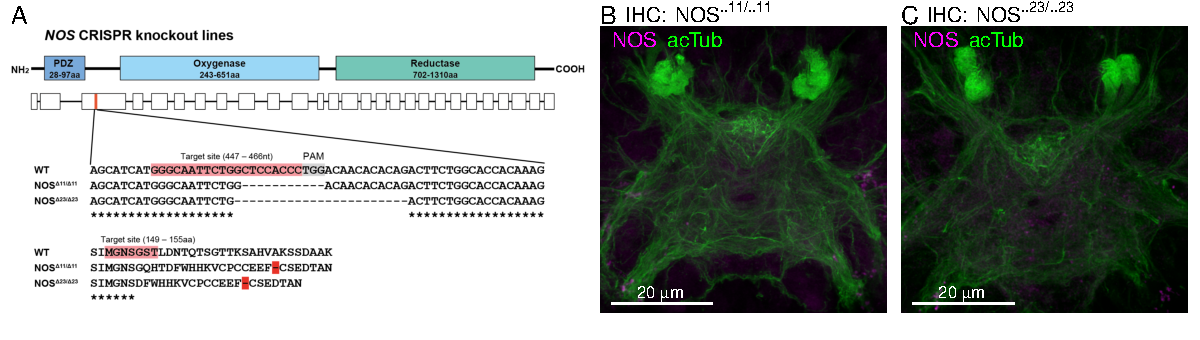
\includegraphics[width=44.44in]{figures/Fig3_sup1} \caption{**Figure 3 -- figure supplement 1. Generation and behavioural characterisation of *NOS* CRISPR knockouts.** (**A**) Top: The domain organisation of *Platynereis* NOS protein and exon/intron structure of the *NOS* gene. Bottom: The genomic locus of *NOS* with the CRISPR target site, wild-type and knockout (NOSΔ11, NOSΔ23) sequences and predicted protein sequences. The PAM sequence is shown in grey, stop codons in red. (**B**) Swimming trajectories of wild type (WT, n=37) and *NOS* mutant (NOSΔ11/Δ11, n=18 and NOSΔ23/Δ23, n=8) two-day-old larvae. All trajectories start at 0 x and y position and time 0 corresponding to 10 sec after the onset of 395 nm stimulation from the side. (**C**)  Vertical displacement in 30 sec bins of wild type and mutant (NOSΔ11 and NOSΔ23) two-day-old larvae stimulated with 395 nm light from the side, 488 nm light from the top and 395 nm light from the top. (**D**) Vertical position of batches of wild type and mutant two-day-old larvae over time under 395 nm UV stimulation. The starting position of each larval trajectory was set to 0. (**E-G**) Swimming speed of batches of wild type and mutant two-day old (E) and three-day-old (F) larvae and L-NAME-treated (NOS inhibitor) three-day-old larvae under 395 nm UV stimulation. <br> Figure 3 -- figure suppmenet 1 -- source data 1-6. Source data for panels B-G.}\label{fig:unnamed-chunk-12}
\end{figure}

\begin{figure}
\includegraphics[width=33.33in]{figures/Fig4_sup1} \caption{**Figure 4 -- figure supplement 1. Cluster analysis of guanylate and adenylate cyclase sequences.** Each node represents one sequence, colour-coded by taxonomy. Connections represent BLAST P-values of <1e-16. NIT-GCs, NIT domain containing guanylate cyclases; membrane-bound GCs, membrane-bound guanylate cyclases; sGCs, soluble guanylate cyclases; ACs, adenylate cyclases.}\label{fig:unnamed-chunk-13}
\end{figure}

\begin{figure}
\includegraphics[width=20.83in]{figures/Fig4_sup2} \caption{**Figure 4 -- figure supplement 2. Maximum-likelihood phylogenetic tree of NIT-domain-containing guanylate cyclases** Membrane-bound and soluble guanylate cyclases (sGC) were included as outgroups. Guanylate cyclases with NIT domains are found in most animal phyla except Porifera, Ctenophora, Urochordata and Chordata. Branch support values indicate UFBoot and aLRT-SH-like values. The expression of *Platynereis* NIT-GC genes in cPRC, INNOS and INRGW cells is indicated on the right side of the tree. The values represent expression based on single-cell sequencing data. Dot size indicates specificity (percent of transcripts expressed in the indicated cell across all cells). Dot colour represents the logarithm of the number of transcripts in the expressing cells. <br> Figure 4 -- figure supplement 2 -- source data 1. GC sequences used for the phylogenetic reconstruction. <br> Figure 4 -- figure supplement 2 -- source data 2. Aligned and trimmed GC sequences used for the phylogenetic reconstruction. <br> Figure 4 -- figure supplement 3 -- source data 3. Tree file of the reconstructed GC phylogeny. }\label{fig:unnamed-chunk-14}
\end{figure}

\begin{figure}
\includegraphics[width=33.33in]{figures/Fig4_sup3} \caption{**Figure 4 -- figure supplement 3. Expression of NIT-GC1 and NIT-GC2 in the cPRCs** (**A**) HCR co-expression analysis of *NIT-GC1* (magenta) and *MLD/pedal-peptide-2 proneuropeptide* (green). Anterior view of a two-day-old larva. Nuclei were stained with DAPI (cyan). **(B, C)** Expression of *NIT-GC2* (magenta) detected by in situ HCR. Anterior (B) and ventral (C) views of a three-day-old larva. Nuclei were stained with DAPI (cyan). (**D**) Immunostaining for NIT-GC1 (magenta) and NOS (green). Anterior view of a two-day-old larva. Acetylated α-tubulin staining (blue) highlights the neuropil and cPRC cilia. **(E, F)** Immunostaining for NIT-GC1 (E) and NIT-GC2 (F) antibodies in larvae injected with NIT-GC1 (E) or NIT-GC2 (F) morpholinos. Acetylated α-tubulin staining (green) highlights the neuropil and cPRC cilia. Anterior view of a two-day-old larva.}\label{fig:unnamed-chunk-15}
\end{figure}

\begin{figure}
\includegraphics[width=27.78in]{figures/Fig5_sup1} \caption{**Figure 5 -- figure supplement 1. On-slide immunostaining and coexpression analysis of *NOS* and *RYamide proneuropeptide* ** (**A**) Schematic diagram of the on-slide immunostaining procedure after Ca^2+^ imaging.(**B-D**) Co-expression analysis by HCR in situ of *NOS* (magenta) and *RYamide proneuropeptide* (green). Anterior view of a two-day-old larva. Nuceli were stained by DAPI (cyan). }\label{fig:unnamed-chunk-16}
\end{figure}

\begin{figure}
\centering
\includesvg{figures/Figure6_fig_Suppl1.svg}
\caption{\textbf{Figure 6 -- figure supplement 1. Simulated
Ca\textsuperscript{2+} traces for parameter sets fitted to individual
Ca\textsuperscript{2+}-recordings collected in wild type, \emph{NOS}
knockout, and \emph{NIT-GC2} morphant larvae.} (\textbf{A-C}) Simulated
Ca\textsuperscript{2+} traces in cPRC (A), INNOS (B) and INRGW (C) cells
in the wild-type condition. (\textbf{D-F}) Simulated
Ca\textsuperscript{2+} traces in cPRC (D), INNOS (E) and INRGW (F) cells
in the \emph{NOS}-knockout condition. (\textbf{G-I}) Simulated
Ca\textsuperscript{2+} traces in cPRC (G), INNOS (H) and INRGW (I) cells
in the \emph{NIT-GC2}-morphant condition. Thin coloured curves indicate
individual recordings (cPRC - purple, INNOS - blue and INRGW - green),
thin grey curves indicate simulated Ca\textsuperscript{2+} traces based
on model parameters fitted to the individual recording, thick coloured
curves indicate averages of the recordings and thick black curves
represent the average of the fits.}
\end{figure}

\begin{figure}
\centering
\includesvg{figures/Figure6_fig_Suppl2.svg}
\caption{\textbf{Figure 6 -- figure supplement 2. Comparison of fits
with different fixed parameter sets when fitting the WT model to
individual recordings from the WT INRGW cells.} Panels A-B, D-E, G-H
(column fixed parameters) show simulated traces of the
Ca\textsuperscript{2+} levels in cPRC and INNOS cells produced by
different fixed parameter sets. Panels C, F and I show individual
recordings fitted to the data from INRGW cells.}
\end{figure}

\begin{figure}
\centering
\includesvg{figures/Figure6_fig_Suppl3.svg}
\caption{\textbf{Figure 6 -- figure supplement 3. Comparison of fits to
the cPRC recordings from NIT-GC2 morphant larvae using the NIT-GC2
morpholino model or the NOS-knockout model.} Thin coloured curves
indicate individual recordings, thin grey curves are simulated
Ca\textsuperscript{2+} traces, thick coloured curves indicate averages
of the recordings and thick black curves represent the mean of the
fits.}
\end{figure}

\begin{figure}
\centering
\includesvg{figures/Figure6_fig_Suppl4.svg}
\caption{\textbf{Figure 6 -- figure supplement 4. Distributions of the
parameter values fitted to the cPRC recordings.} Violin plots (grey
lines) are kernel density estimates of the underlying distributions;
computed using the Matlab function \emph{ksdensity} with default
settings, i.e., using normal kernel function, plots are trimmed to the
observed range of data. Markers represent individual parameter values,
white markers indicate medians, vertical grey bars indicate
interquartile range (Q25 to Q75), and the dashed line indicates the
value 1. Where violin plots are not shown, these parameters are
associated with terms/equations that are excluded from the fitting
procedure (see Methods for details).}
\end{figure}

\begin{figure}
\centering
\includesvg{figures/Figure6_fig_Suppl5.svg}
\caption{\textbf{Figure 6 -- figure supplement 5. Pairwise correlations
between parameters of the WT model fitted to WT cPRC recordings}
Parameters associated with the \(C_R\) equation are not included (see
Methods for details). Panels on the diagonal show kernel density
estimates of the distributions of the individual parameters; computed
using Matlab function \emph{ksdensity} with default settings, i.e.,
using normal kernel function, plots are trimmed to the observed range of
data. The other panels show kernel density estimates of bivariate
distributions of pairs of parameters (heatmaps; darker colours indicate
higher density). Also shown using markers are the values of the
individual parameter combinations.}
\end{figure}

\end{document}
